\documentclass[a4paper, 11pt]{article}
\usepackage{graphicx} % Required for inserting images
\usepackage{multirow}
\usepackage[utf8]{inputenc}
\usepackage[top=1.5cm, bottom=1.5cm, left=1.5cm, right=1.5cm]{geometry}
\usepackage[T1]{fontenc}
\usepackage{amsmath}
\usepackage{amsthm}
\usepackage{amsfonts}
\usepackage{amssymb}
\usepackage{adjustbox}
\usepackage{array}
\usepackage{algorithm}
\usepackage{algpseudocode}
\usepackage{siunitx} % Pour la notation scientifique
\usepackage{graphicx}
\usepackage{subcaption} % Pour les sous-figures
\usepackage{booktabs} % Pour de meilleurs tableaux
\usepackage{subcaption}  % Nécessaire pour les sous-figures
\usepackage[utf8]{inputenc}
\usepackage[french]{babel}
\usepackage{hyperref}
\usepackage{natbib}
\usepackage{enumitem}
\usepackage{bbm}
% Configure siunitx to handle units correctly
\sisetup{detect-all, separate-uncertainty=true}


% Définition des unités manquantes pour siunitx
% Utilisez les unités standard de siunitx : \kilogram, \metre, \second, \knot existent déjà ou utilisez \si{kg}, \si{m}, \si{s}, \si{kt}
% Si besoin, décommentez la ligne suivante pour la définition de \knot si elle n'existe pas dans votre version de siunitx :
% \DeclareSIUnit\knot{kt}
\usepackage{subcaption} % Pour les sous-figures
\usepackage{booktabs} % Pour de meilleurs tableaux
\usepackage{subcaption}  % Nécessaire pour les sous-figures
\usepackage{tocloft} % Pour personnaliser la table des matières
\usepackage{lmodern}
\usepackage{siunitx}
% Définition du niveau subsubsubsection
\makeatletter
% Créer un nouveau compteur pour subsubsubsection
\newcounter{subsubsubsection}[subsubsection]
% Format du numéro : ex. 1.2.3.4
\renewcommand\thesubsubsubsection{\thesubsubsection.\@arabic\c@subsubsubsection}
% Définition de la commande subsubsubsection
\newcommand\subsubsubsection{\@startsection{subsubsubsection}{4}{\z@}%
    {-1.5ex \@plus -0.2ex \@minus -0.2ex}% Espace avant
    {0.5ex \@plus 0.2ex}% Espace après
    {\normalfont\normalsize\bfseries}}% Style de la police
% Commande pour le marquage dans le texte (optionnel)
\newcommand{\subsubsubsectionmark}[1]{}
% Ajouter subsubsubsection à la table des matières
\makeatother

% Définir les commandes tocloft pour subsubsubsection
\makeatletter
% Définir l'entrée dans la table des matières
\newcommand{\l@subsubsubsection}{\@dottedtocline{4}{7em}{4em}}
% Définir les commandes pour l'indentation et la largeur du numéro
\newcommand{\cftsubsubsubsecindent}{7em}
\newcommand{\cftsubsubsubsecnumwidth}{4em}
\makeatother

% Configurer la profondeur de la table des matières
\setcounter{tocdepth}{4}
\setcounter{secnumdepth}{4}

\begin{document}

\begin{titlepage}
\begin{center}
    
\includegraphics[width=0.3\linewidth]{Logo-toulouse-inp-N7.png}
\end{center}
    \centering
    \vspace*{3in} % Ajuste la hauteur pour centrer verticalement
    \Huge \textbf{Rapport de Metamodelisation} \\[1cm] % Titre
    \Large {Axel OLOUGOUNA, Qian WANG}\\ % Auteur
            {Ayoub CHOUKRI, Minh Duy NGUYEN} \\
    \Large Juin 2025 % Date
    \vfill
\end{titlepage}

\newpage

\tableofcontents

\newpage

\section{Introduction}
La conception d’un avion commercial est un défi multidisciplinaire nécessitant l’optimisation de nombreux paramètres sous des contraintes strictes de performance, de sécurité et de réglementation. Les simulations numériques, bien que précises, sont coûteuses en temps et en ressources, rendant leur usage intensif difficile dans un cadre industriel. Pour surmonter cette limitation, la métamodélisation offre une solution efficace en construisant des modèles surrogates capables d’approximer le comportement des simulateurs à un coût computationnel réduit. \newline

Ce rapport s’intéresse à l’optimisation d’un avion de 150 passagers environ volant à Mach 0.78, en étudiant deux configurations de propulsion : kérosène/turbofan et hydrogène/turbofan. L’objectif principal est de minimiser la masse maximale au décollage (\textbf{mtom}) tout en respectant des contraintes opérationnelles, telles que la longueur de piste au décollage, la vitesse d’approche ou l’envergure. Les paramètres de conception incluent la poussée, le nombre de passagers, la surface alaire et le rapport d’aspect, tandis que des paramètres incertains, liés à l’aérodynamique, la propulsion et la structure, sont pris en compte dans les analyses avancées. \newline

Le rapport est structuré comme suit : le \textbf{Problème 1} explore la construction et l’optimisation d’un métamodèle pour résoudre un problème d’optimisation déterministe. Le \textbf{Problème 2} introduit les incertitudes via des distributions de probabilité, tandis que le \textbf{Problème 3} propose trois méthodes (développement de Taylor, surrogate direct et surrogate local itératif) pour intégrer ces incertitudes dans l’optimisation. 

\section{Conditions d'expérience}

On veut optimiser un avion d'environ 150 passagers qui vole à Mach 0.78 en utilisant différents moteurs et différents type de carburant. Pour cela, on va vouloir trouver les paramètres de conception qui minimise le maximum de la masse au décollage (\textbf{mtom}).
Ci-après, la présentation des différents paramètres sur lesquels nous allons travailler.


\subsection{Paramètres de Conception}
Les paramètres de conception sont :
\begin{itemize}
    \item La poussée statique maximale au niveau de la mer (\(100 \, \text{kN} \leq \textbf{slst} \leq 200 \, \text{kN}\), par défaut : \(150 \, \text{kN}\)),
    \item Le nombre de passagers (\(120 \leq {\textbf{n\_pax}} \leq 180\), par défaut : \(150\)),
    \item La surface des ailes (\(100 \, \text{m}^2 \leq \textbf{area} \leq 200 \, \text{m}^2\), par défaut : \(180 \, \text{m}^2\)),
    \item Le rapport d'aspect de l'aile (\(5 \leq \textbf{ar} \leq 20\), par défaut : \(9\)).
\end{itemize}

\subsection{Contraintes Opérationnelles}
Les contraintes opérationnelles sont :
\begin{itemize}
    \item La longueur de piste au décollage (\(\textbf{tofl} \leq 1900 \, \text{m}\)),
    \item La vitesse d'approche (\(\textbf{vapp} \leq 135 \, \text{kt}\)),
    \item La vitesse verticale (\(\textbf{vz} \geq 300 \, \text{ft/min}\)),
    \item L'envergure de l'aile (\(\textbf{envergure} \leq 40 \, \text{m}\)),
    \item La longueur de l'aile (\(\textbf{longueur} \leq 45 \, \text{m}\)),
    \item La marge de carburant (\(\textbf{fm} \geq 0\%\)).
\end{itemize}

\subsection{Paramètres Incertains}
Dans les problèmes 2 et 3, certains paramètres sont considérés comme incertains. Ces paramètres incertains sont modélisés comme des variables aléatoires définies par des distributions de probabilité :

\begin{table}[H]
\centering
\begin{tabular}{l c c c}
\toprule
\textbf{Variable} & \textbf{Distribution} & \textbf{Type de carburant} & \textbf{Type de moteur} \\ 
\midrule
\( \textbf{gi} \) & \( T(0.35, 0.4, 0.405) \) & hydrogène\_liquide & Tous \\
\( \textbf{vi} \) & \( T(0.755, 0.800, 0.805) \) & hydrogène\_liquide & Tous \\
\( \textbf{aef} \) & \( T(0.99, 1.0, 1.03) \) & Tous & Tous \\
\( \textbf{cef} \) & \( T(0.99, 1.0, 1.03) \) & Tous & Tous \\
\( \textbf{sef} \) & \( T(0.99, 1.0, 1.03) \) & Tous & Tous \\
\( \textbf{fc\_pwd} \) & \( T(0.8, 1, 1.02) \) & hydrogène\_liquide & électroventilateur \\
\( \textbf{bed} \) & \( U(400, 700) \) & batterie & Tous \\
\bottomrule
\end{tabular}
\caption{Paramètres incertains avec leurs distributions de probabilité, type de carburant et type de moteur. \( T(\text{minimum}, \text{mode}, \text{maximum}) \) représente la distribution triangulaire, et \( U(\text{minimum}, \text{maximum}) \) représente la distribution uniforme.}
\end{table}

Voici un tableau récapitulatif des significations probables des variables incertaines, basé sur le contexte de la conception aéronautique :


\begin{center}
\begin{tabular}{lcp{8cm}}
\toprule
Variable & Signification probable \\
\midrule
\( g1 \) & Facteur de gravité ou rapport de poussée spécifique pour \( liquide\_H2 \). \\
\( v1 \) & Vitesse critique ou croisière normalisée pour \( liquide\_H2 \). \\
\( sef \) & Efficacité structurelle, applicable à tous. \\
\( cef \) & Efficacité du coefficient de traînée, applicable à tous. \\
\( aef \) & Efficacité aérodynamique globale, applicable à tous. \\
\( fc\_pwd \) & Facteur de consommation par watt pour \( liquide\_H2 \) et electrofan. \\
\( bed \) & Capacité de la batterie en Wh/kg pour systèmes à batterie. \\
\bottomrule
\end{tabular}
\end{center}

\subsection{Cas d'études}
On va prendre deux configurations pour étudier résoudre divers problèmes.

\begin{table}[H]
\centering
\begin{tabular}{l c c c}
\toprule
\textbf{} & \textbf{Type de carburant} & \textbf{Type de moteur} & \textbf{Portée de conception (km)} \\
\midrule
Use Case 1 & Kérosène & Turbofan & 5500 \\
Use Case 2 & Hydrogène & Turbofan & 5500 \\
\bottomrule
\end{tabular}
\caption{Cas d'utilisation avec leurs types de carburant, types de moteur et portée de conception.}
\end{table}


\section{Problème 1 - Métamodèle et optimisation}

\subsection{Présentation du problème}
Le but de ce problème est de créer un métamodèle de $\hat{f}:x\mapsto \hat{f}(x)=f(x,u_{\text{default}})$ ($x$ représentant l'ensemble des paramètres de conception et $u_{\text{default}}$ la valeur par défaut pour les paramètres incertains) pour approximer l'objectif et les contraintes du problème de design. Ensuite, nous utiliserons le métamodèle pour résoudre un problème d'optimisation en faisant varier la plage d'entrée des paramètres.

\subsection{Création du métamodèle}
Étant donné que nous disposons de quatre variables d’entrée et que le simulateur en temps réel est coûteux en temps de calcul, nous nous limitons à 20 échantillons pour constituer notre métamodèle. \newline

Pour construire notre métamodèle, on utilise la fonction \texttt{SurrogateDiscipline} de \textbf{GEMSEO} avec comme régresseur (\textbf{RBFRegressor}, \textbf{MOERegressor}, etc). \newline

\subsubsection{Différents choix de modèles surrogates}
\subsubsubsection{RBFRegressor}
\label{RBF}
Le régresseur \textbf{RBFRegressor} approxime la fonction cible \(\hat{f}(x)\) par une combinaison linéaire de fonctions à base radiale gaussiennes :
\[
\hat{f}(x) = \sum_{i=1}^N w_i \phi(\| x - c_i \|) + b,
\]
où \(\phi(r) = \exp\left(-\frac{r^2}{2\varepsilon^2}\right)\) est la fonction radiale, \( c_i \) sont les centres (points d'entraînement), \( w_i \) les poids, \( b \) un biais, et \(\varepsilon\) un paramètre de lissage. \newline

\subsubsubsection{MOERegressor}
\label{MOE}
Le régresseur \textbf{MOERegressor} est une mixture de plusieurs models de régressions. Dans un premier temps, il crée K clusters avec les données en entrées. Puis il crée sur chaque cluster des modèles de régression.
La sortie pour une entrée devient la somme pondérée des prédictions de chaque modèle de régression.

\[
y = \sum_{k=1}^{K} w_k(x) f_k(x),
\]

On peut avoir deux types de classification : 
\begin{itemize}
    \item La classification dure: dans ce cas, les poids sont définis par \[
    w_k(x) = \mathbbm{1}_{x \in C_k} ,
    \] et on ne garde que l'apport de la classe où l'entrée est classifiée.
    \item La classification douce: dans ce cas, les poids sont définis par \[
    w_k(x) = \mathbb{P}(x \in C_k) 
    \] où \( \mathbb{P}(x \in C_k)  \) est la probabilité que l'entrée appartienne au cluster \( k\). \newline
\end{itemize} 

\subsubsection{Création d'un domaine d'expériences}
Un plan d’expériences basé sur un échantillonnage Latin Hypercube Sampling (LHS) optimisé est généré pour échantillonner l’espace des paramètres de conception défini par les paramètres \(\texttt{slst}\), \(\texttt{n\_pax}\), \(\texttt{area}\), et \(\texttt{ar}\). 


\subsubsection{Coefficient de détermination $R^2$}
Le coefficient de détermination \( R^2 \) mesure la qualité de l’ajustement d’un modèle en quantifiant la proportion de la variance totale des données expliquée par le modèle. Mathématiquement, il est défini comme suit :
\[
R^2 = 1 - \frac{\sum_{i=1}^n (y_i - \hat{y}_i)^2}{\sum_{i=1}^n (y_i - \bar{y})^2},
\]
où \( y_i \) est la valeur observée, \( \hat{y}_i \) est la valeur prédite par le modèle, \( \bar{y} \) est la moyenne des valeurs observées, et \( n \) est le nombre d’observations. Un \( R^2 \) proche de 1 indique que le modèle explique presque toute la variabilité des données, tandis qu’un \( R^2 \) proche de 0 indique un mauvais ajustement.

\subsection{Optimisation du métamodèle}

Une fois le métamodèle construit, on procède à l'optimisation en l'utilisant à la place du modèle direct car il est moins coûteux en temps de calcul et donc plus facile à optimiser.
On crée donc un scénario en se basant sur le métamodèle.
Une fois l'optimisation finie, on s'assure que les contraintes sont respectés sur le modèle direct.

\subsection{Résultats obtenus}

\subsubsection{Use Case 1}

Dans un premier temps on réalise le métamodèle sur UC1 en utilisant RBFRegressor. On obtient pour un $R^2 = 1$ pour les différentes variables du modèle sur les données d'entraînement. Sur les données de test (100 échantillons), on obtient un $R^2 = 0.88$ pour la variable \textbf{tofl} et un $R^2 \geq 0.94 $ pour toutes les autres variables. Cela signifie que le métamodèle a bien approximé notre simulateur. \newline 

La figure \ref{fig:pu1u1optim} ci-dessous présente les résultats de l'optimisation du métamodèle pour l'UC 1.


\begin{figure}[H]
    \centering
    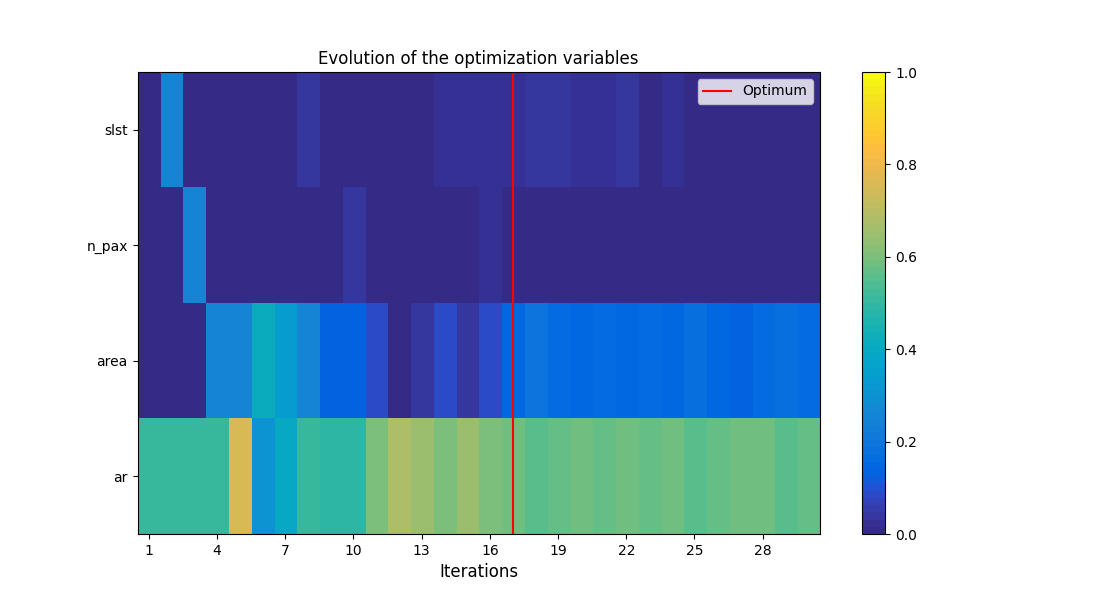
\includegraphics[width=0.49\linewidth]{Images_case_1/p1u1_evol_optim_variables2.png}
    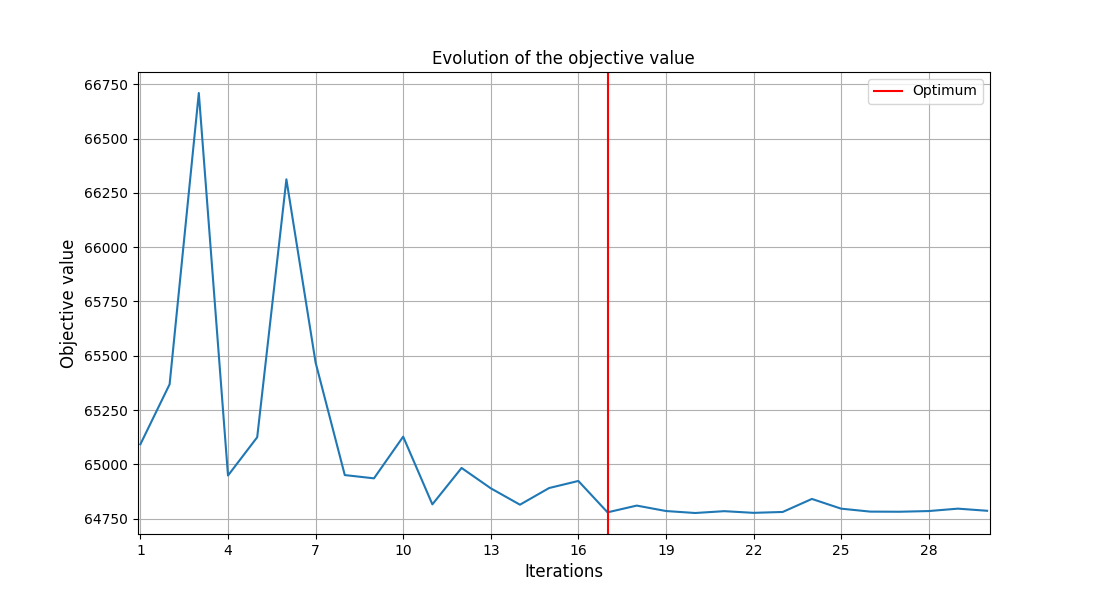
\includegraphics[width=0.49\linewidth]{Images_case_1/p1u1_evol_obj_val2.png}
    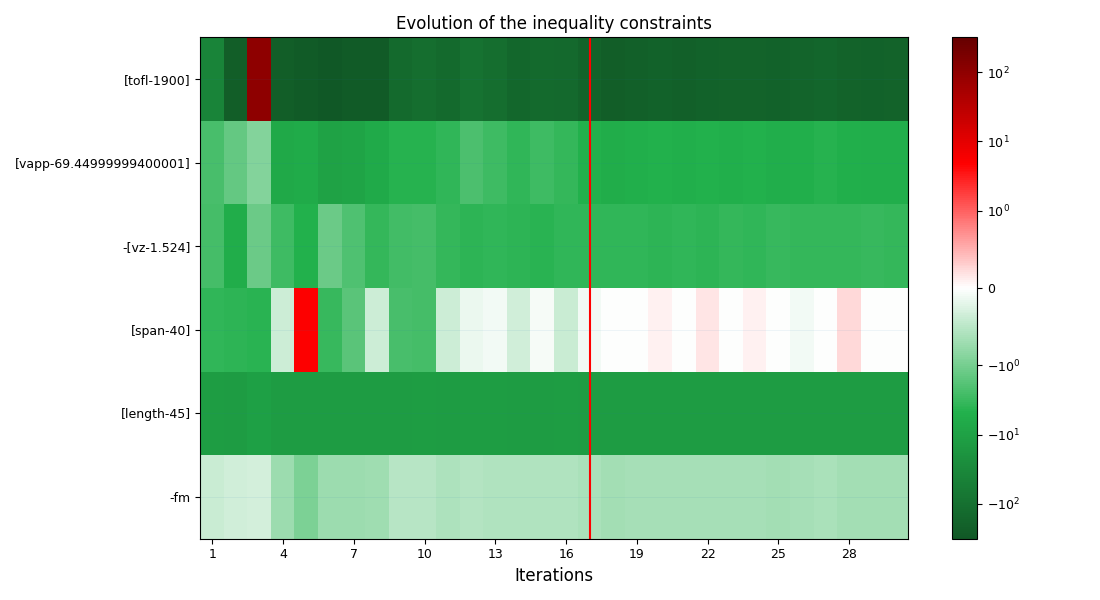
\includegraphics[width=0.49\linewidth]{Images_case_1/p1u1_evol_ineq_const2.png}
    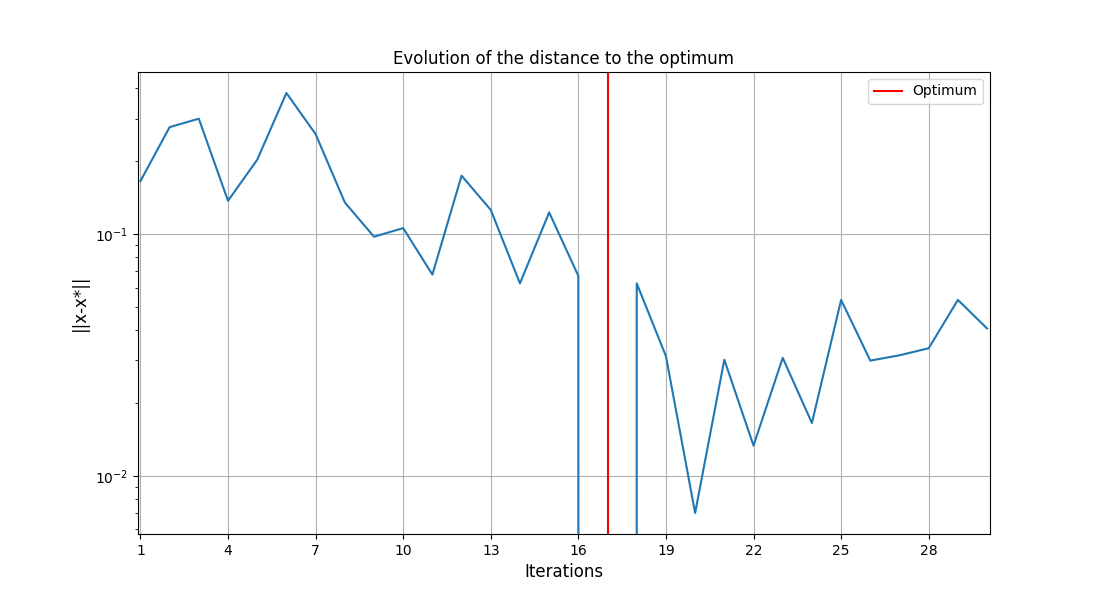
\includegraphics[width=0.49\linewidth]{Images_case_1/p1u1_evol_dist_to_opt2.png}
    \caption{Évolution de l'optimisation pour UC1}
    \label{fig:pu1u1optim}
\end{figure}

Les résultats de l'optimisation pour le cas UC1 montrent une convergence satisfaisante vers une solution optimale après 19 itérations.

\begin{itemize}

    \item \textbf{Evolution de l'optimisation des variables:} Cette heatmap illustre l'évolution des variables d'optimisation (\texttt{slst, n\_pax, ar}) sur les itérations. Les couleurs vont du bleu (valeurs basses) au jaune (valeurs hautes). On constate que les paramètres (\texttt{slst}, \texttt{n\_pax}, \texttt{area}, \texttt{ar} ) se stabilisent autour de la $17^{eme}$ itération, marquée par la ligne rouge indiquant l'optimum.

    \item \textbf{Evolution de la valeur de l'objectif:} La valeur objective (\texttt{mtom}) diminue progressivement de 78000 kg à environ 64000 kg, confirmant une réduction effective de la masse totale au décollage. Elle se stabilise après l'optimum à l'itération 24, marqué par une ligne rouge verticale.

    \item \textbf{Evolution des contraintes d'inéqualités:} Ce graphique en heatmap montre l'évolution des contraintes \texttt{(tofl, vapp, vz, span, length, fm)} sur les itérations. Les contraintes d'inégalité restent majoritairement respectées (donc de couleur verte, inversement ) au cours des itérations, bien qu'on constate quelques fois des pics temporaires (notamment pour \texttt{span} et \texttt{tofl}).
    
    \item \textbf{Evolution de la distance à l'optimum:} Cette représente la distance (en norme) à l'optimum au fil des itérations.  La distance diminue progressivement, avec des fluctuations, indiquant une convergence vers l'optimum, marqué par une ligne rouge verticale à l'itération 19. La distance à l'optimum, initialement de l'ordre de $10^0$, chute à $10^{-2}$ vers la fin, validant la convergence de l'algorithme. 

\end{itemize}

La vérification avec le modèle direct confirme la cohérence des résultats.
Les paramètres après optimisation sont les suivants:
\begin{itemize}
    \item \texttt{slst} : 102669.61243896
    \item \texttt{n\_pax} : 120
    \item \texttt{area} : 114.20991753
    \item \texttt{ar} : 13.70699063
\end{itemize}

On affiche maintenant les avions par défaut et celui obtenu après optimisation.

\begin{figure}[H]
    \centering
    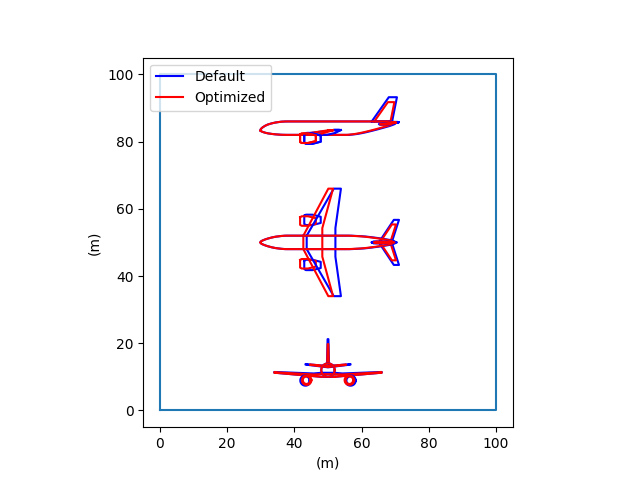
\includegraphics[width=0.8\linewidth]{Images_case_1/p1u1_plots_of_the_aircrafts.png}
    \caption{Les différents avions}
    \label{fig:p1u1avions}
\end{figure}

On constate que l'avion obtenu possède des dimensions plus petites que celui par défaut.

\subsubsection{Cas d'étude 2}

Dans un premier temps on utilise le RBFRegresssor pour réaliser le métamodèle. Mais on se rend compte que les contraintes après optimisation ne sont pas vérifiées pour le modèle direct. On cherche donc le régresseur qui fonctionne et au final on choisit MOERegressor avec une classification de type dure. \newline

On obtient pour un $R^2 = 1$ pour les différentes variables du modèle sur les données d'entraînement. Sur les données de test (100 échantillons), on obtient un $R^2 = 0.88$ pour la variable \texttt{tofl} et un $R^2 \geq 0.94 $ pour toutes les autres variables. Cela signifie que le métamodèle a bien approximé notre simulateur.\newline

Il faut noter que le paramètre \texttt{tofl} est un paramètre dont le contrainte n'était pas vérifiée avec d'autres régresseurs. \newline

La figure \ref{fig:pu1u2optim} ci-dessous présente les résultats de l'optimisation du métamodèle pour l'UC 2.

\begin{figure}[H]
    \centering
    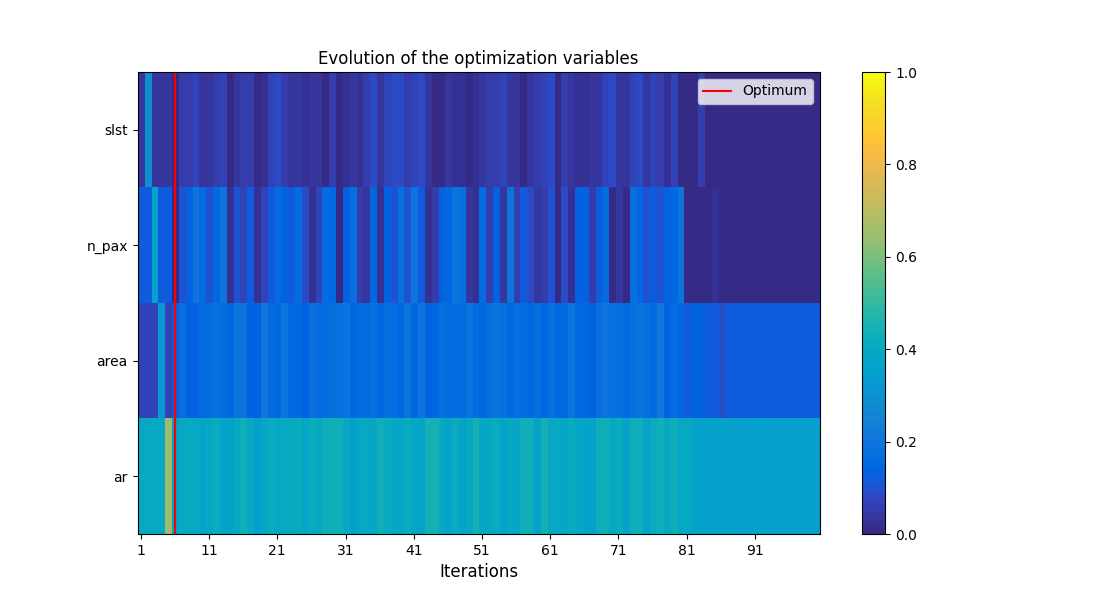
\includegraphics[width=0.49\linewidth]{Images_case_2/p1u2_evol_optim_variables2.png}
    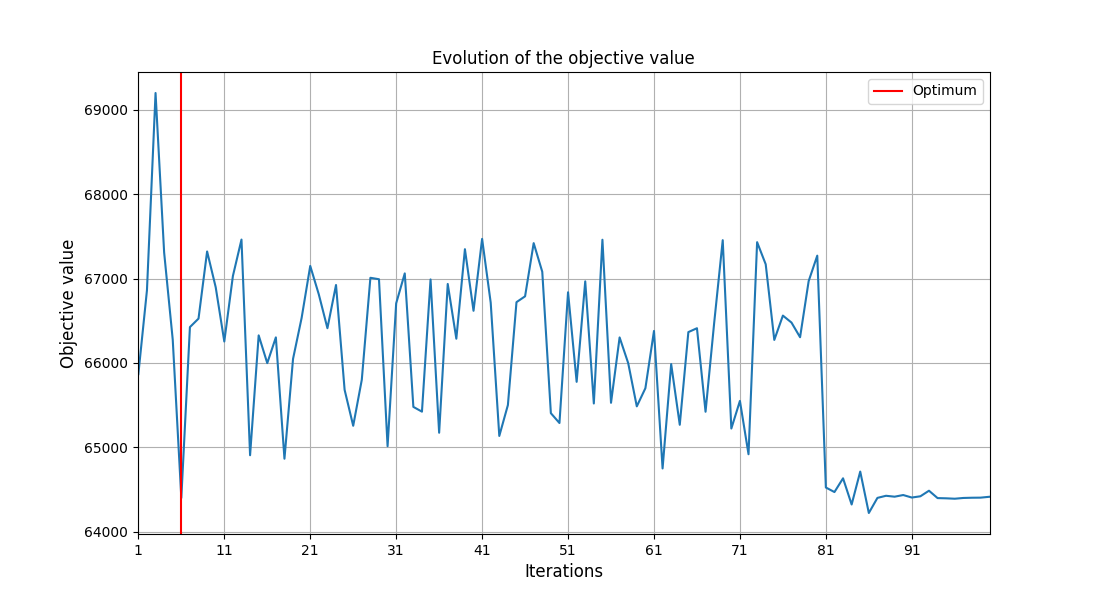
\includegraphics[width=0.49\linewidth]{Images_case_2/p1u2_evol_obj_val2.png}
    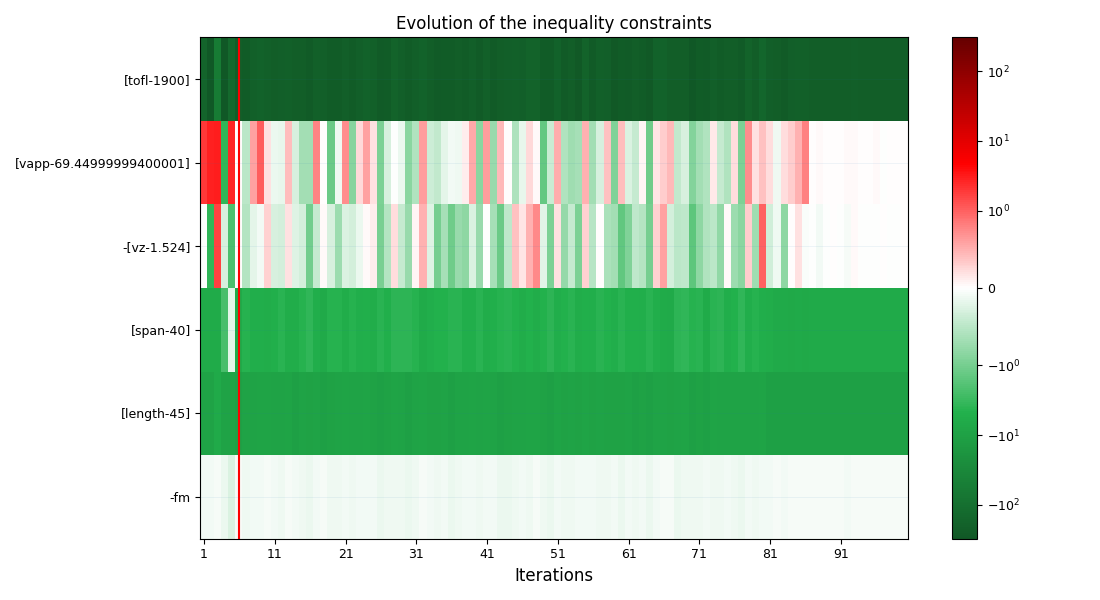
\includegraphics[width=0.49\linewidth]{Images_case_2/p1u2_evol_ineq_const2.png}
    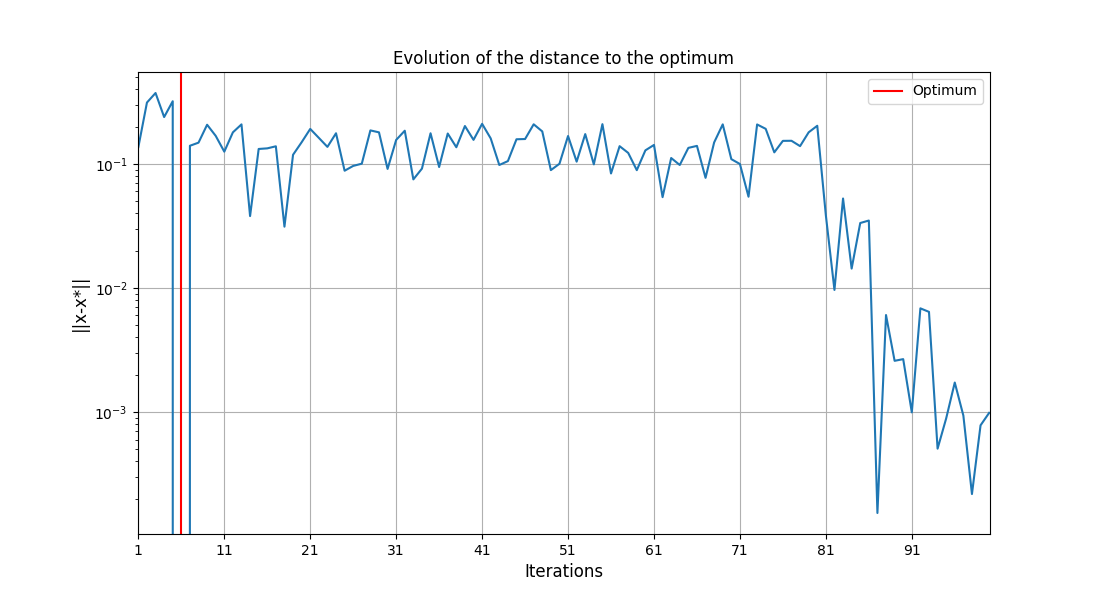
\includegraphics[width=0.49\linewidth]{Images_case_2/p1u2_evol_dist_to_opt2.png}
    \caption{Évolution de l'optimisation pour UC2}
    \label{fig:pu1u2optim}
\end{figure}


Les résultats de l'optimisation pour le cas UC1 montrent une convergence satisfaisante vers une solution optimale après 5 itérations.

\begin{itemize}

    \item \textbf{Evolution de l'optimisation des variables:} Cette heatmap illustre l'évolution des variables d'optimisation \texttt{(slst, n\_pax, ar)} sur les itérations. Les couleurs vont du bleu (valeurs basses) au jaune (valeurs hautes). On constate que les paramètres (\texttt{slst}, \texttt{n\_pax}, \texttt{area},\texttt{ar}) se stabilisent autour de la $5^{eme}$ itération, marquée par la ligne rouge indiquant l'optimum.

    \item \textbf{Evolution de la valeur de l'objectif:} La valeur objective (\texttt{mtom}) diminue progressivement de 69000 kg à environ 64000 kg, confirmant une réduction effective de la masse totale au décollage. Elle est atteinte à l'itération 5 mais se stabilise après l'itération 81.

    \item \textbf{Evolution des contraintes d'inéqualités:} Ce graphique en heatmap montre l'évolution des contraintes (tofl, vapp, vz, span, length, fm) sur les itérations. Les contraintes d'inégalité restent majoritairement respectées au cours des itérations, bien qu'on constate quelques fois des pics temporaires (notamment pour \texttt{vapp} et \texttt{vz}).
    
    \item \textbf{Evolution de la distance à l'optimum:} Cette représente la distance(en norme) à l'optimum au fil des itérations (de 1 à 100).  On constate qu'elle fluctue énormément augmentent encore même après avoir attendu l'optimum à la 5ème itération.

\end{itemize}

La vérification avec le modèle direct confirme la cohérence des résultats.
Les paramètres après optimisation sont les suivants:
\begin{itemize}
    \item \textbf{slst} : 100000.
    \item \textbf{n\_pax} : 120
    \item \textbf{area} : 112.48807812
    \item \textbf{ar} : 10.34990761
\end{itemize}
On a une $\texttt{mtom} = 63402.36070368503$. On affiche maintenant les avions par défaut et celui obtenu après optimisation.

\begin{figure}[H]
    \centering
    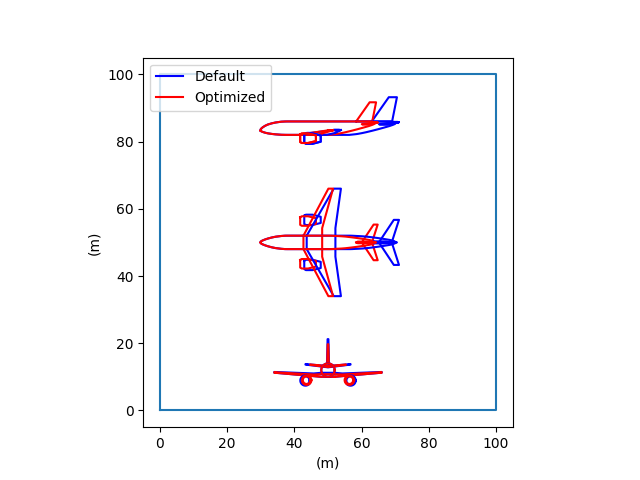
\includegraphics[width=0.8\linewidth]{Images_case_2/p1u2_plots_of_the_aircrafts.png}
    \caption{Les différents avions}
    \label{fig:p1u1avions}
\end{figure}

On constate que l'avion obtenu possède ici aussi des dimensions plus petites que celui par défaut.


%% Partie Ayoub Début
% Creating the section for Problem 2
\section{Problème 2 - Modélisation par substitut et quantification des incertitudes}

Dans cette partie, nous développerons une approche pour quantifier les incertitudes liées aux choix technologiques dans le processus de conception d’un avion. L’objectif est de créer des modèles de substitut pour approximer la fonction \( u \mapsto f(\mathbf{x}, \mathbf{u}) \), où \( \mathbf{x} \) représente les paramètres de conception et \( \mathbf{u} \) les paramètres incertains. Nous examinerons deux cas spécifiques : \( f(\mathbf{x}_{\text{default}}, \mathbf{u}) \) avec les paramètres de conception à leurs valeurs par défaut, et \( f(\mathbf{x}_{\text{opt}}, \mathbf{u}) \) avec les paramètres optimisés. Ces modèles seront utilisés pour propager les incertitudes et analyser leur impact.

\subsection{Approche proposée}

Notre méthodologie pour quantifier les incertitudes dans la conception d’un avion repose sur l’utilisation de la bibliothèque GEMSEO pour modéliser et analyser le système. Les étapes suivantes décrivent l’approche mise en œuvre :

\begin{enumerate}
    \item \textbf{Création de modèles de substitut :}
    \begin{enumerate}
        \item \textbf{Création d’un plan d’expériences (DoE) :} Un plan d’expériences basé sur un échantillonnage Latin Hypercube Sampling (LHS) optimisé est généré pour échantillonner l’espace des paramètres incertains \( \mathbf{u} \). Cela permet de collecter des données d’entraînement représentatives pour les modèles de substitut, en utilisant la fonction \texttt{sample\_disciplines} de GEMSEO.
        \item \textbf{Entraînement des modèles de substitut :} Des modèles de substitut sont construits pour \( f(\mathbf{x}_{\text{default}}, \mathbf{u}) \) et \( f(\mathbf{x}_{\text{opt}}, \mathbf{u}) \) à l’aide de la méthode \texttt{RBFRegressor} (Radial Basis Function Regressor) implémentée via la classe \texttt{SurrogateDiscipline} de GEMSEO, assurant une approximation précise des relations entrée-sortie.
    \end{enumerate}

    \item \textbf{Estimation des quantités d’intérêt :}
    \begin{enumerate}
        \item \textbf{Échantillonnage Monte Carlo :} Les paramètres incertains \( \mathbf{u} \), définis par leurs distributions de probabilité (par exemple, triangulaires pour \( g1 \), \( v1 \), \( sef \), \( cef \), \( aef \), \( fc\_pwd \), et uniforme pour \( bed \)), sont échantillonnés à l’aide de simulations Monte Carlo pour générer un grand nombre d’échantillons représentatifs.
        \item \textbf{Estimation statistique :} À partir des échantillons, les modèles de substitut sont utilisés pour estimer les moyennes, variances, coefficients de variation et autres statistiques des sorties \( y \) (par exemple, \texttt{mtom}, \texttt{tofl}, \texttt{vz}, \texttt{fm}, \texttt{vapp}), permettant d’évaluer l’impact des incertitudes.
    \end{enumerate}

    \item \textbf{Analyse de sensibilité :} Les indices de Sobol sont calculés pour quantifier l’influence de chaque paramètre incertain \( \mathbf{u} \) sur les sorties du système. Cette analyse est réalisée à l’aide des outils de GEMSEO, avec des visualisations générées via \texttt{sobol.plot} pour les variables \texttt{mtom}, \texttt{tofl}, \texttt{vz}, \texttt{fm}, et \texttt{vapp}, mettant en évidence les contributions relatives des paramètres incertains.
\end{enumerate}

Cette approche, appuyée par les fonctionnalités de GEMSEO telles que \texttt{AutoPyDiscipline}, \texttt{DesignSpace}, et \texttt{MDOScenario}, permet une modélisation robuste des interactions multidisciplinaires et une quantification efficace des incertitudes dans le processus de conception aéronautique.


\subsection{Use Case 1}


Pour créer un modèle de substitut permettant d’approximer la fonction \( u \mapsto f(\mathbf{x}, \mathbf{u}) \), nous avons suivi une approche systématique utilisant la bibliothèque GEMSEO. Les étapes détaillées sont décrites ci-dessous, suivies d’une évaluation des performances du modèle.

\subsubsection{Construction du modèle de substitut}

\begin{enumerate}
    \item \textbf{Définition de l’espace des paramètres incertains :} Un espace de paramètres incertains \( \mathbf{u} \) est défini à l’aide de la classe \texttt{MyUncertainSpace}, héritant de \texttt{ParameterSpace} de GEMSEO. Trois paramètres incertains (\texttt{cef}, \texttt{aef}, \texttt{sef}) sont modélisés par des distributions triangulaires avec les paramètres suivants : minimum = 0.99, mode = 1, maximum = 1.03, utilisant \texttt{OTTriangularDistribution} d’OpenTURNS.

    \item \textbf{Plan d’expériences (DoE) :} Un ensemble d’entraînement est généré en échantillonnant l’espace des paramètres incertains avec la méthode LHS OPT (\texttt{OT\_LHS\_OPT}), produisant 20 échantillons pour les sorties \texttt{mtom}, \texttt{tofl}, \texttt{vz}, \texttt{span}, \texttt{length}, \texttt{fm}, et \texttt{vapp}. Ces échantillons sont obtenus via la fonction \texttt{sample\_disciplines} de GEMSEO, avec une graine fixée à 38 pour garantir la reproductibilité.
    

    \item \textbf{Entraînement du modèle :} Le modèle de substitut est construit à l’aide de la classe \texttt{SurrogateDiscipline} avec la méthode \texttt{RBFRegressor} (Radial Basis Function Regressor), configurée avec un paramètre \texttt{epsilon = 100}. Ce modèle est entraîné sur l’ensemble de données généré, permettant une approximation des relations entre les paramètres incertains et les sorties.

    \item \textbf{Évaluation des performances :} Un ensemble de test est généré avec 200 échantillons en utilisant un plan factoriel complet (\texttt{OT\_FULLFACT}), avec une graine fixée à 318, pour évaluer la précision du modèle de substitut sur des données indépendantes.
\end{enumerate}

\subsubsection{Coefficient de détermination \( R^2 \)}

Dans notre cas, les valeurs de \( R^2 \) sont calculées pour les ensembles d’entraînement et de test à l’aide de la classe \texttt{R2Measure} de GEMSEO. Les résultats sont visualisés sous forme de diagrammes en barres pour chaque sortie (\texttt{mtom}, \texttt{tofl}, \texttt{vz}, \texttt{span}, \texttt{length}, \texttt{fm}, \texttt{vapp}), comparant les performances sur les données d’entraînement et de test.

\begin{figure}[H]
    \centering
    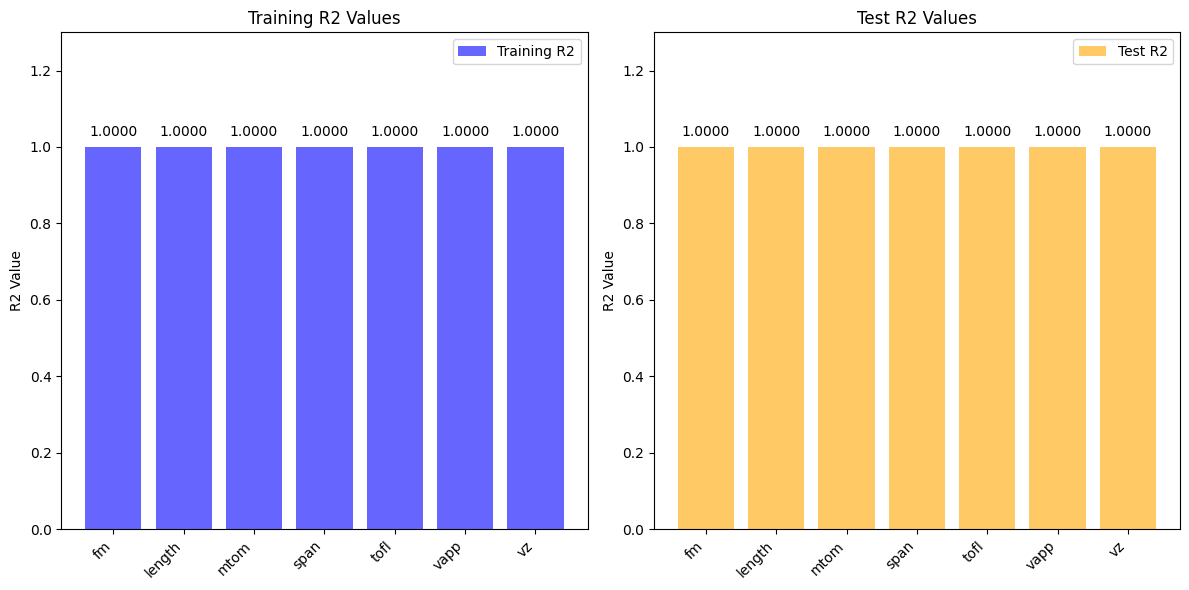
\includegraphics[width=0.8\textwidth]{Images_Ayoub/Problem2/UseCase1/Surrogate/R2/R2.png}
    \caption{Comparaison des valeurs de \( R^2 \) pour l’entraînement (à gauche) et le test (à droite) pour chaque sortie.}
    \label{fig:r2_plot}
\end{figure}

\subsubsection{Résultats de l’entraînement}
Le modèle de substitut a été entraîné avec succès en utilisant seulement 20 points d’échantillonnage, atteignant des valeurs de \( R^2 \) proches de 1 pour presque toutes les sorties (\texttt{mtom}, \texttt{tofl}, \texttt{vz}, \texttt{span}, \texttt{length}, \texttt{fm}, \texttt{vapp}). Ces résultats indiquent une excellente capacité du modèle à capturer les relations entre les paramètres incertains et les sorties, même avec un ensemble d’entraînement limité.


\subsubsection{Estimation des quantités d’intérêt}

Dans cette partie, on s'interesse à l'estimation des quantités d'intérêt comme la moyenne, la variance, le coefficient de variation et les quantiles des sorties du modèle de substitut. Et ce, en injectant les lois de probabilité des paramètres incertains dans le modèle. \newline

Ces estimations vont permettre de quantifier les incertitudes liées aux choix technologiques dans le processus de conception d’un avion.

\subsubsubsection{Génération des échantillons}

Pour générer les échantillons des paramètres incertains, nous avons utilisé la méthode Monte Carlo. Les distributions de probabilité des paramètres incertains \( \mathbf{u} \) sont définies comme suit :
\begin{itemize}
    \item \( sef \) : Distribution triangulaire \( T(0.99, 1.1, 1.03) \)
    \item \( cef \) : Distribution triangulaire \( T(0.99, 1.1, 1.03) \)
    \item \( aef \) : Distribution triangulaire \( T(0.99, 1.1, 1.03) \)
\end{itemize}



Nous avons généré $20000$ échantillons pour chaque paramètre incertain en utilisant la méthode Monte Carlo. Ces échantillons sont stockés dans un tableau de taille \( 5000 \times 3 \), où chaque colonne correspond à un paramètre incertain. \newline

Une idée intéressante serait de visualiser la distribution des échantillons générés pour chaque paramètre incertain, et aussi de visualiser la distribution des sorties du modèle de substitut pour les échantillons générés. Cela permettrait de mieux comprendre la variabilité des sorties en fonction des incertitudes des paramètres.


\subsubsubsection{Distribution des sorties du modèle de substitut}
Pour visualiser la distribution des sorties du modèle de substitut, nous avons utilisé les échantillons générés précédemment. Chaque sortie du modèle de substitut est calculée en injectant les échantillons des paramètres incertains dans le modèle. Les sorties considérées sont \( \texttt{mtom} \), \( \texttt{tofl} \), \( \texttt{vz} \), \( \texttt{span} \), \( \texttt{length} \), \( \texttt{fm} \), et \( \texttt{vapp} \).



\begin{figure}[h]
    \centering
    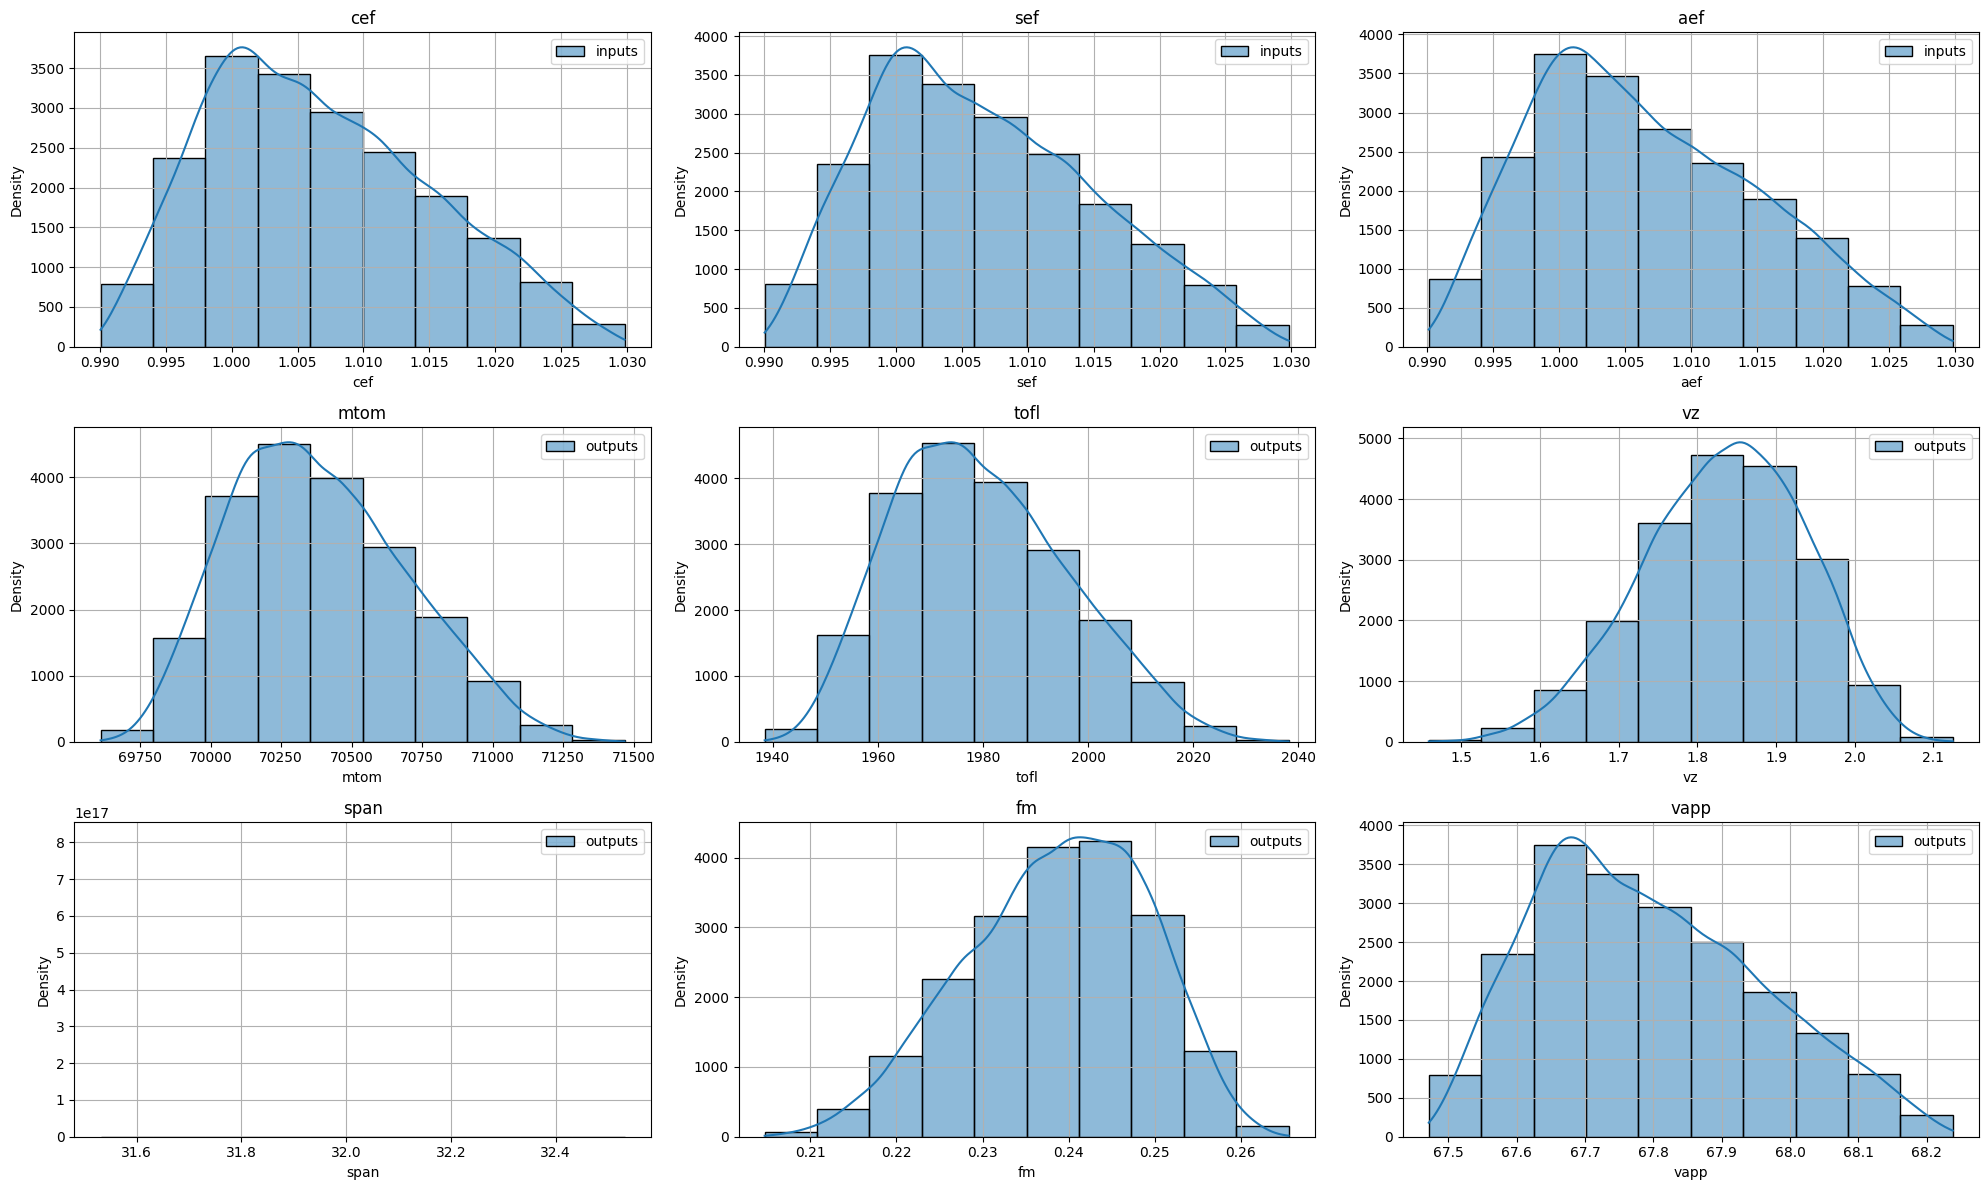
\includegraphics[width=0.95\textwidth]{Images_Ayoub/Problem2/UseCase1/Estimating_Quantities/Input_Output_Distributions/Input_Output_Distributions.png}
    \caption{Distribution des échantillons générés pour chaque paramètre incertain (en haut) et distribution des sorties du modèle de substitut (en bas) pour les 20000 échantillons.}
    \label{fig:input_output_distributions}
\end{figure}


\paragraph{Analyse des distributions}

La figure ci-dessous présente, dans les trois premiers graphiques, les distributions de probabilité des paramètres incertains injectés dans le modèle de substitut : \( \texttt{cef} \), \( \texttt{sef} \), et \( \texttt{aef} \). Ces paramètres suivent tous une loi triangulaire définie par \( T(0.99, 1.1, 1.03) \), avec un mode à 1.03. Cette distribution reflète une incertitude modérée autour d’une valeur nominale, avec une concentration importante des échantillons autour de ce mode.

Les autres histogrammes représentent les distributions des sorties du modèle de substitut obtenues via simulation Monte Carlo. On peut faire les observations suivantes :

\begin{itemize}
    \item \textbf{mtom} (masse maximale au décollage) : distribution légèrement asymétrique à droite, concentrée entre $69750$ et $71500$. Cela indique une variabilité notable, avec un risque de valeurs élevées non négligeable.
    
    \item \textbf{tofl} (longueur de piste au décollage) : distribution centrée, presque symétrique, autour de 1900. La variabilité est faible, ce qui traduit une bonne stabilité face aux incertitudes.
    
    \item \textbf{vz} (vitesse ascensionnelle) : distribution symétrique et bien concentrée autour de 1.7 à 1.9. Cela traduit une réponse régulière du modèle et peu sensible aux incertitudes d’entrée.
    
    \item \textbf{span} (envergure) : distribution quasi-plate, indiquant une variable probablement constante ou très peu influencée par les paramètres incertains. Cela peut refléter une hypothèse de conception fixant cette grandeur.
    
    \item \textbf{fm} (figure of merit) : distribution légérement assymétrique vers la gauche, centrée vers 0.24.
    
    \item \textbf{vapp} (vitesse d’approche) : distribution légèrement asymétrique à droite, concentrée entre $67.5$ et $68.2$. Cela montre une certaine sensibilité à l’incertitude, mais sans dérive excessive.
\end{itemize}


\subsubsubsection{Estimation des moyennes et variances et Coefficients de variation}


Le coefficient de variation (CV) d'une variable $X_i$ est défini comme l'écart-type \(\sqrt{\text{Var}(X_i)}\) divisé par la valeur absolue de l'espérance \(|{\mathbb{E}(X_i)}|\), exprimé mathématiquement par :

\begin{equation}
\text{CV} = \frac{\sqrt{\text{Var}(X_i)}}{|{\mathbb{E}(X_i)}|}
\end{equation}
\begin{table}[h]et
\centering
\caption{Paramètres de l'aéronef : moyenne, variance et coefficient de variation}
\begin{tabular}{l S[table-format=1.2e2] S[table-format=1.6e2] S[table-format=2.3]}
\toprule
\textbf{Paramètre} & \textbf{Moyenne} & \textbf{Variance} & \textbf{CV (\%)} \\
\midrule
MTOM (\si{\kilo\gram}) & 7.04e4 & 9.67e4 & 0.442 \\
TOFL (\si{\meter}) & 1.98e3 & 2.77e2 & 0.841 \\
Vz (\si{\meter\per\second}) & 1.83e0 & 1.06e-2 & 5.609 \\
Span (\si{\meter}) & 3.20e1 & 5.05e-29 & 0.000 \\
Length (\si{\meter}) & 3.70e1 & 0.00e0 & 0.000 \\
FM & 2.39e-1 & 1.10e-4 & 4.389 \\
Vapp (\si{\knot}) & 6.78e1 & 2.66e-2 & 0.241 \\
CEF & 1.01e0 & 7.18e-5 & 0.842 \\
AEF & 1.01e0 & 7.24e-5 & 0.845 \\
SEF & 1.01e0 & 7.15e-5 & 0.840 \\
\bottomrule
\end{tabular}
\end{table}

\begin{figure}[H]
\centering
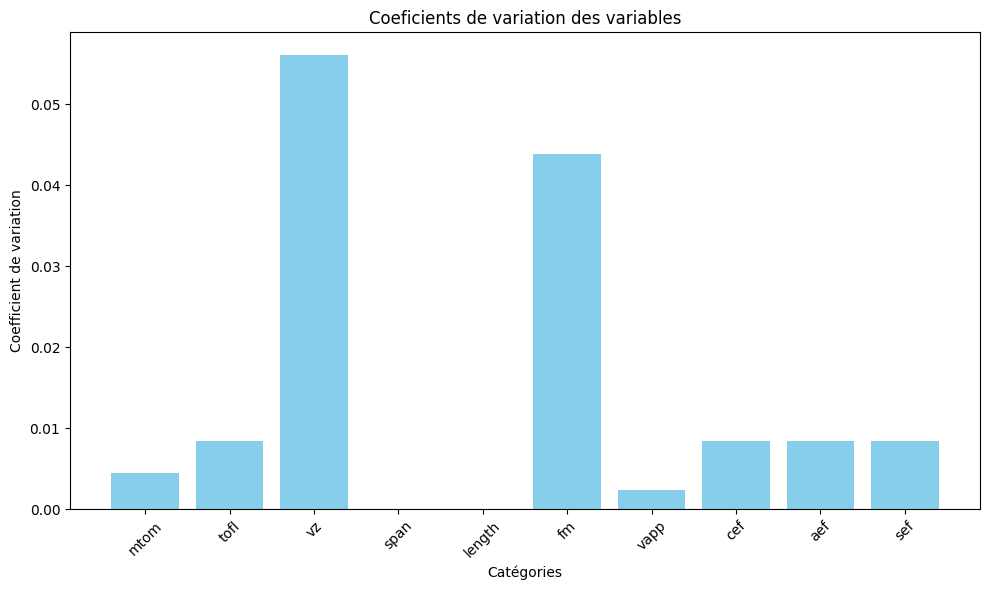
\includegraphics[width=0.8\textwidth]{Images_Ayoub/Problem2/UseCase1/Estimating_Quantities/Coefficient_De_Variation/Coefficient_Variation.png}
\caption{Coefficients de variation des différentes variables}
\label{fig:image1}
\end{figure}
On remarque que la vitesse verticale (\textbf{vz}) , ainsi que la marge de carburant (\textbf{fm}) ont les coefficients de variation les plus élevés ( $5$\%, $4.8$\%). Ce qui pourrait poser des problèmes dans la vérification des contraintes opérationnelles. Pour les autres variables, le coefficient de variation reste dans l'ordre de $1\%$

\begin{figure}[H]
\centering
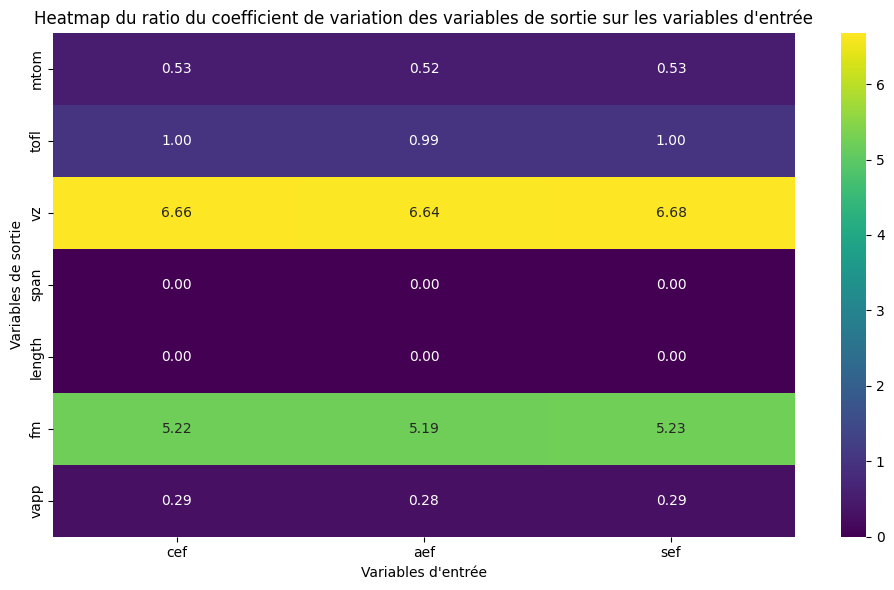
\includegraphics[width=0.8\textwidth]{Images_Ayoub/Problem2/UseCase1/Estimating_Quantities/Coefficient_De_Variation/Ratio_Coefficient_Variation.png}
\caption{Heatmap du ratio du coefficient de variation}
\label{fig:image2}
\end{figure}



\subsubsection{Indices de Sobol}
Les indices de Sobol sont un outil essentiel en analyse de sensibilité, permettant de quantifier la contribution de chaque variable d'entrée à la variance de la sortie d'un modèle. Pour une fonction \( f(\mathbf{x}) \) avec un vecteur d'entrée \( \mathbf{x} = (x_1, x_2, \dots, x_d) \), la variance totale \( V \) de la sortie peut être décomposée en contributions des effets principaux des variables et de leurs interactions :
\[
V = \sum_{i=1}^d V_i + \sum_{1 \leq i < j \leq d} V_{ij} + \cdots + V_{1,2,\dots,d},
\quad \text{avec} \quad
V_i = \mathrm{Var}\big[\mathbb{E}[Y \mid x_i]\big],
\quad
V_{ij} = \mathrm{Var}\big[\mathbb{E}[Y \mid x_i, x_j]\big] - V_i - V_j.
\]

Ici, \( V_i \) représente la variance due à l'effet principal de la variable \( x_i \), tandis que des termes comme \( V_{ij} \) capturent les interactions entre \( x_i \) et \( x_j \).  \newline

L'indice de Sobol de premier ordre pour une variable \( x_i \) est défini comme :
\[
S_i = \frac{V_i}{V} = \frac{\mathrm{Var}\big[\mathbb{E}[Y \mid x_i]\big]}{\mathrm{Var}[Y]}.
\]

Cet indice mesure la contribution directe de \( x_i \) à la variance totale, sans les interactions. Pour évaluer l'influence globale de \( x_i \), y compris ses interactions avec les autres variables, on utilise l'indice de Sobol total \( S_{T_i} \), donné par :
\[
S_{T_i} = 1 - \frac{V_{-i}}{V} = \sum_{E \text{ tel que } i \in E} \frac{V_E}{V}
\]

où \( V_{-i} \) est la variance lorsque \( x_i \) est fixée et que toutes les autres variables varient. Les indices de Sobol sont normalisés, la somme des indices de premier ordre et des termes d'interaction valant 1, ce qui en fait un outil idéal pour classer l'importance des variables dans des modèles complexes.


\subsubsubsection{Indices de Sobol pour les sorties du modèle de substitut}


Les indices de Sobol sont calculés pour les sorties du modèle de substitut afin d'évaluer l'importance relative des paramètres incertains sur chaque sortie. Les résultats sont présentés dans la figure ci-dessous, où chaque barre représente l'indice de Sobol pour un paramètre donné et une sortie spécifique. \newline



\begin{figure}[H]
    \centering
    \begin{subfigure}[b]{0.45\textwidth}
        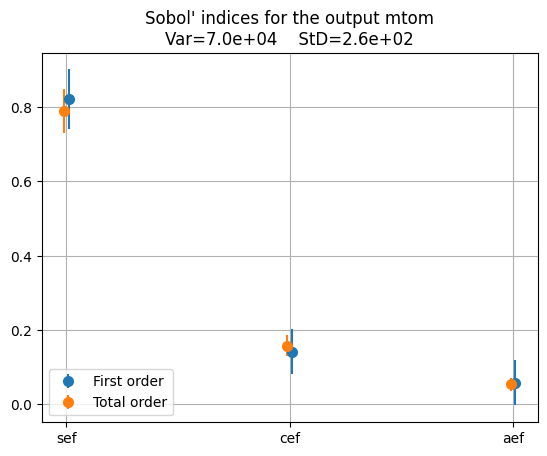
\includegraphics[width=\textwidth]{Images_Ayoub/Problem2/UseCase1/Sobol_Indices/mtom.png}
        \caption{MTOM}
        \label{fig:mtom}
    \end{subfigure}
    \hfill
    \begin{subfigure}[b]{0.45\textwidth}
        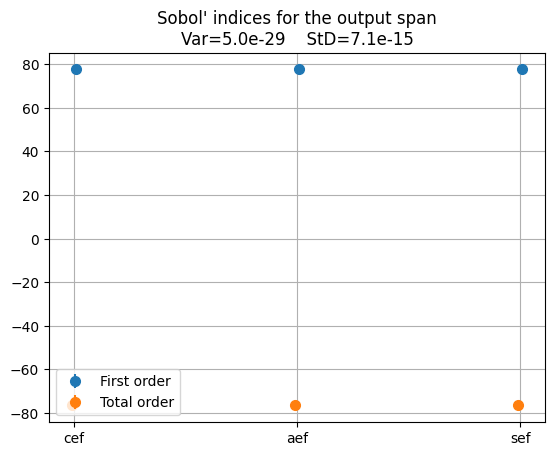
\includegraphics[width=\textwidth]{Images_Ayoub/Problem2/UseCase1/Sobol_Indices/span.png}
        \caption{Span}
        \label{fig:span}
    \end{subfigure}

    \vspace{10pt} % Espacement vertical entre les lignes

    \begin{subfigure}[b]{0.45\textwidth}
        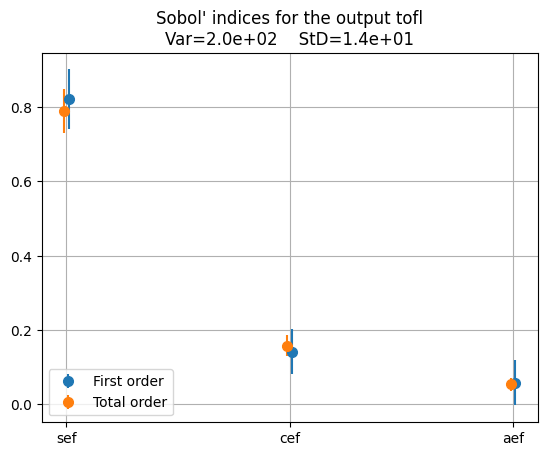
\includegraphics[width=\textwidth]{Images_Ayoub/Problem2/UseCase1/Sobol_Indices/tofl.png}
        \caption{TOFL}
        \label{fig:tofl}
    \end{subfigure}
    \hfill
    \begin{subfigure}[b]{0.45\textwidth}
        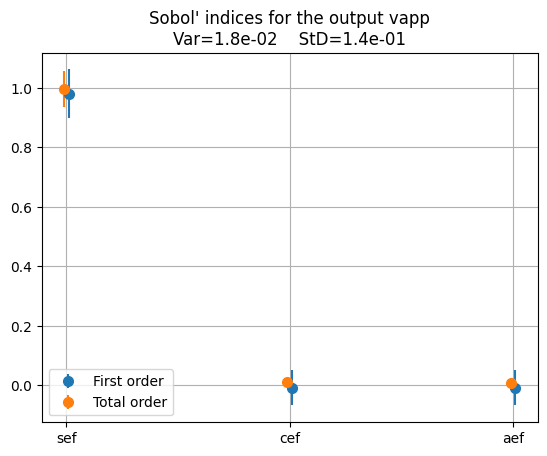
\includegraphics[width=\textwidth]{Images_Ayoub/Problem2/UseCase1/Sobol_Indices/vapp.png}
        \caption{Vapp}
        \label{fig:vapp}
    \end{subfigure}

    \vspace{10pt} % Espacement vertical entre les lignes

    \begin{subfigure}[b]{0.45\textwidth}
        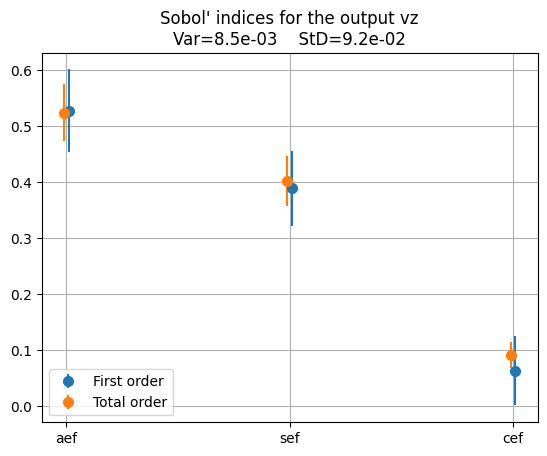
\includegraphics[width=\textwidth]{Images_Ayoub/Problem2/UseCase1/Sobol_Indices/vz.png}
        \caption{Vz}
        \label{fig:vz}
    \end{subfigure}
    \hfill
    \begin{subfigure}[b]{0.45\textwidth}
        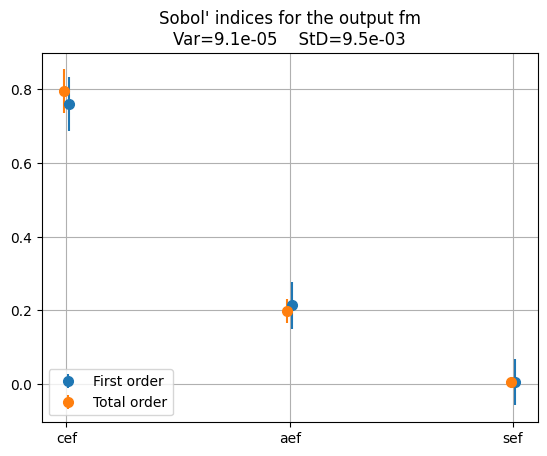
\includegraphics[width=\textwidth]{Images_Ayoub/Problem2/UseCase1/Sobol_Indices/fm.png}
        \caption{FM}
        \label{fig:fm}
    \end{subfigure}

    \caption{Indices de Sobol pour différentes sorties du modèle de substitut.}
    \label{fig:sobol_indices}
\end{figure}


\begin{itemize}
    \item Les sorties (MTOM, Span, TOFL, Vz, Vapp) dépendent principalement des paramètres set, ctf, aef et aet, comme indiqué par les indices de Sobol.
    \item Pour MTOM, l'indice de Sobol total est significativement plus élevé que l'indice de premier ordre, suggérant une forte interaction entre les paramètres.
    \item Pour Span, les indices totaux (Var=5.0e-29, STD=7.1e-15) dépassent les indices de premier ordre, indiquant des effets d'interaction notables.
    \item TOFL montre une dépendance marquée aux indices totaux (Var=2.0e-02, STD=1.4e-01), avec des interactions plus importantes que les effets individuels.
    \item Vz et Vapp présentent des indices totaux modérés (Var=9.5e-03, STD=9.5e-03 pour Vapp), mais les différences avec les indices de premier ordre restent mineures, suggérant une dépendance plus directe.
    \item Globalement, les indices de Sobol totaux sont souvent supérieurs aux indices de premier ordre, révélant que les interactions entre paramètres jouent un rôle clé dans la variabilité des sorties.
\end{itemize}


% Use case 2 

\subsection{Cas d'étude 2}


Le Use Case 2 est lié à l'etude de l'avion à hydrogène. Trois nouvelles variables incertaines ont été introduites : rapport de poussée spécifique (\( g1 \)), vitesse de croisière (\( v1 \)) et facteur de charge (\( fc\_pwd \)). \newline

Ces variables sont modélisées par des distributions triangulaires, avec les paramètres suivants :

\begin{center}
\begin{tabular}{lccccc}
\toprule
Variable & Distribution & Type de carburant & Type de moteur \\
\midrule
\( g1 \) & \( T(0.35, 0.4, 0.405) \) & liquide\_H2 & All \\
\( v1 \) & \( T(0.755, 0.800, 0.805) \) & liquide\_H2 & All \\
\( sef \) & \( T(0.99, 1.1, 1.03) \) & All & All \\
\( cef \) & \( T(0.99, 1.1, 1.03) \) & All & All \\
\( aef \) & \( T(0.99, 1.1, 1.03) \) & All & All \\
\( fc\_pwd \) & \( T(0.8, 1.1, 1.02) \) & liquide\_H2 & electrofan \\
\( bed \) & \( U(400, 700) \) & battery & All \\
\bottomrule
\end{tabular}
\end{center}



\subsubsection{Modèle de substitut pour le Use Case 2}

Les mêmes étapes que pour le Use Case 1 ont été suivies pour créer un modèle de substitut permettant d’approximer la fonction \( u \mapsto f(\mathbf{x}, \mathbf{u}) \) pour le Use Case 2. Les paramètres incertains ont été définis, un plan d’expériences a été généré, et le modèle de substitut a été entraîné en utilisant la classe \texttt{SurrogateDiscipline} avec la méthode \texttt{RBFRegressor}.

%% Affichage des R2





\begin{figure}[H]
    \centering
    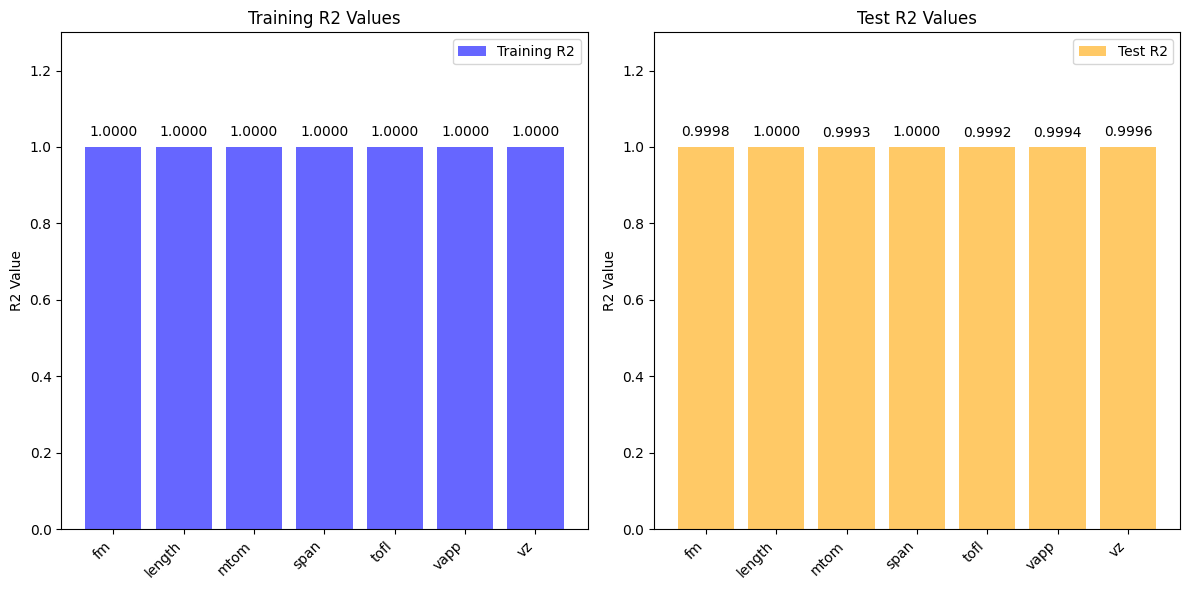
\includegraphics[width=0.8\textwidth]{Images_Ayoub/Problem2/UseCase2/Surrogate/R2/R2.png}
    \caption{Comparaison des valeurs de \( R^2 \) pour l’entraînement (à gauche) et le test (à droite) pour chaque sortie.}
    \label{fig:r2_plot_usecase2}
\end{figure}



\subsubsection{Résultats de l’entraînement}
Le modèle de substitut a été entraîné avec succès en utilisant seulement 20 points d’échantillonnage, atteignant des valeurs de \( R^2 \) proches de 1 pour presque toutes les sorties (\texttt{mtom}, \texttt{tofl}, \texttt{vz}, \texttt{span}, \texttt{length}, \texttt{fm}, \texttt{vapp}). Ces résultats indiquent une excellente capacité du modèle à capturer les relations entre les paramètres incertains et les sorties, même avec un ensemble d’entraînement limité.


\subsubsection{Estimation des quantités d’intérêt}

Pour le Use Case 2, nous avons également généré des échantillons des paramètres incertains en utilisant la méthode Monte Carlo. Les distributions de probabilité des paramètres incertains sont les mêmes que celles définies précédemment, avec l’ajout des nouvelles variables \( g1 \) et \( v1 \).


\begin{figure}[H]
    \centering
    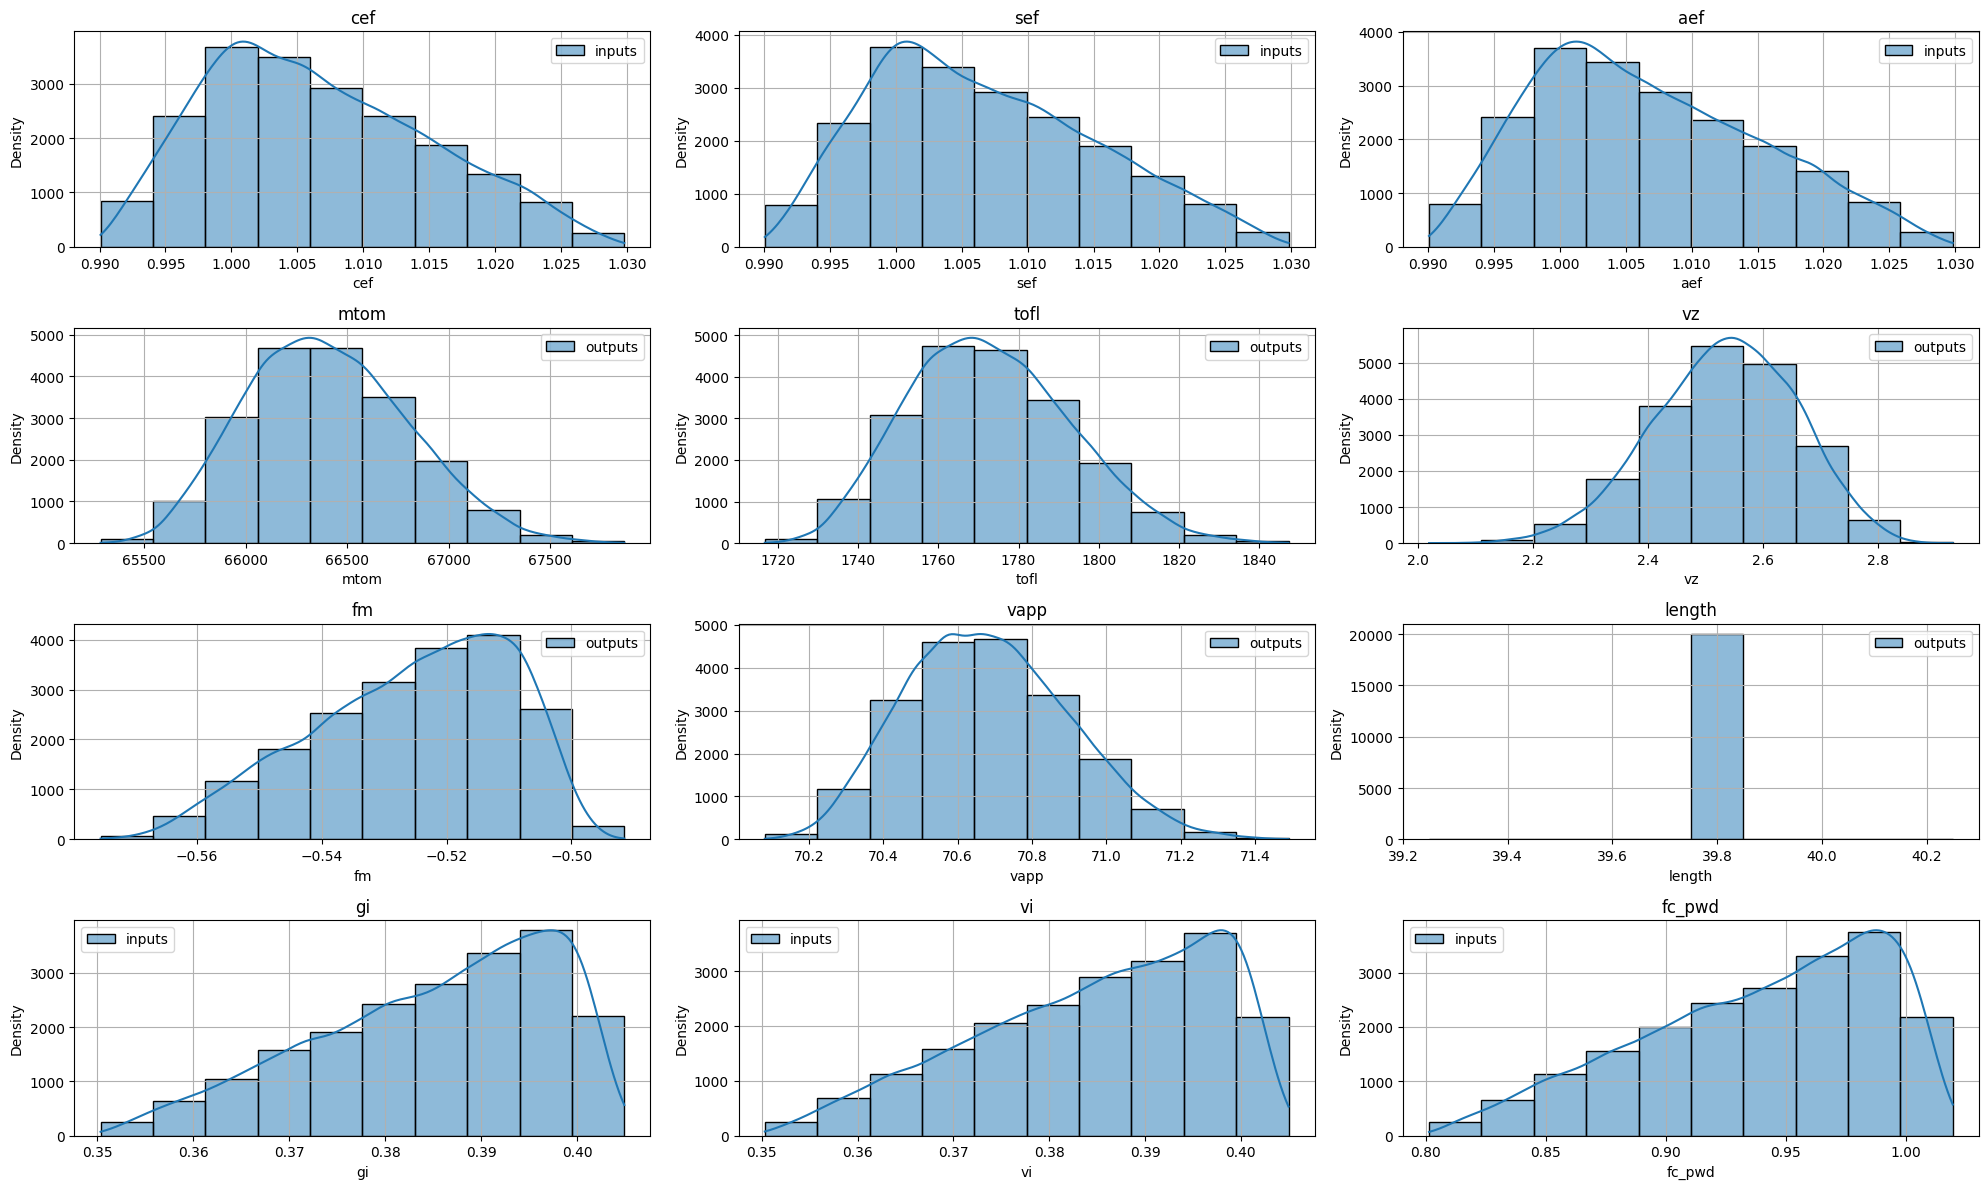
\includegraphics[width=0.95\textwidth]{Images_Ayoub/Problem2/UseCase2/Estimating_Quantities/Input_Output_Distributions/Input_Output_Distributions.png}
    \caption{Distribution des échantillons générés pour chaque paramètre incertain (en haut) et distribution des sorties du modèle de substitut (en bas) pour les 20000 échantillons.}
    \label{fig:input_output_distributions_usecase2}
\end{figure}

\paragraph{Analyse des distributions}

La figure ci-dessous présente, dans les trois premiers graphiques, les distributions de probabilité des paramètres incertains injectés dans le modèle de substitut : \( \texttt{cef} \), \( \texttt{sef} \), et \( \texttt{aef} \). Ces paramètres suivent tous une loi triangulaire définie par \( T(0.99, 1.1, 1.03) \), avec un mode à 1.03. Cette distribution reflète une incertitude modérée autour d’une valeur nominale de 1.03, avec une concentration importante des échantillons autour de ce mode et des queues s’étendant jusqu’à 0.99 et 1.1, indiquant une variabilité contrôlée.

Les autres histogrammes représentent les distributions des sorties du modèle de substitut obtenues via simulation Monte Carlo. On peut faire les observations suivantes :

\begin{itemize}
    \item \textbf{mtom} (masse maximale au décollage) : Distribution légèrement asymétrique à droite, centrée entre 66000 et 67000, avec une queue s’étendant jusqu’à 72000. Cette variabilité notable suggère un risque de valeurs élevées non négligeable, probablement influencée par les incertitudes des paramètres d’entrée.
    
    \item \textbf{tofl} (longueur de piste au décollage) : Distribution presque symétrique, centrée autour de 1780 à 1900, avec une densité maximale proche de 1800. La faible dispersion indique une bonne stabilité du modèle face aux incertitudes d’entrée.
    
    \item \textbf{vz} (vitesse ascensionnelle) : Distribution symétrique et bien concentrée entre 1.7 et 1.9, avec un pic autour de 1.8. Cette régularité reflète une réponse robuste et peu sensible aux variations des paramètres incertains.
    
    \item \textbf{fm} (figure of merit) : Distribution gaussienne centrée autour de -0.52 à -0.50, avec une densité maximale près de -0.51. La forme étroite et symétrique indique une stabilité élevée du critère de performance malgré les incertitudes.
    
    \item \textbf{vapp} (vitesse d’approche) : Distribution légèrement asymétrique à droite, concentrée entre 70.2 et 71.2, avec un pic autour de 70.8. Cette légère dissymétrie suggère une sensibilité modérée aux incertitudes, sans dérive excessive.
    
    \item \textbf{length} (longueur de l’avion) : Distribution symétrique et très étroite, centrée autour de 39.6 à 39.8, avec une densité maximale près de 39.7. La faible variabilité témoigne d’une excellente prédictibilité.
    
    \item \textbf{gi} : Distribution légèrement asymétrique à droite, concentrée entre 0.36 et 0.40, avec un pic autour de 0.38. Cette variabilité modérée indique une influence mesurée des paramètres incertains.
    
    \item \textbf{vi} : Distribution symétrique et bien concentrée entre 0.37 et 0.39, avec un pic autour de 0.38. Cette stabilité suggère une faible sensibilité aux variations d’entrée.
    
    \item \textbf{fc\_pwd} : Distribution symétrique et centrée entre 0.90 et 0.95, avec un pic autour de 0.92. La faible dispersion reflète une robustesse et une prédictibilité élevées.
\end{itemize}


\subsubsubsection{Estimation des moyennes et variations et Coefficients de variation}

De la même façon que pour le Use Case 1, nous avons calculé les moyennes, variances et coefficients de variation, l'inter-quartile pour les sorties du modèle de substitut. Les résultats sont présentés dans le tableau ci-dessous :

\begin{table}[h]
\centering
\caption{Paramètres de l'aéronef : moyennes, variances, coefficients de variation et intervalles interquartiles corrigés}
\begin{tabular}{l S[table-format=1.2e2] S[table-format=1.6e2] S[table-format=2.3] S[table-format=1.2e2]}
\toprule
\textbf{Paramètre} & \textbf{Moyenne} & \textbf{Variance} & \textbf{CV (\%)} & \textbf{IQ} \\
\midrule
MTOM (\si{\kilo\gram}) & 6.6402e4 & 1.5904e5 & 0.601 & 0.0042 \\
TOFL (\si{\meter}) & 1.7728e3 & 4.0639e2 & 1.137 & 0.0080 \\
Vz (\si{\meter\per\second}) & 2.534e0 & 1.5410e-2 & 4.900 & 0.0341 \\
Span (\si{\meter}) & 3.2031e1 & 5.0487e-29 & 0.000 & 0.0000 \\
Length (\si{\meter}) & 3.975e1 & 0.0000e0 & 0.000 & 0.0000 \\
FM & -5.2553e-1 & 2.5221e-4 & 3.022 & -0.0228 \\
Vapp (\si{\knot}) & 7.0681e1 & 4.7853e-2 & 0.309 & 0.0022 \\
CEF & 1.0066e0 & 7.1774e-5 & 0.842 & 0.0063 \\
AEF & 1.0067e0 & 7.2565e-5 & 0.846 & 0.0064 \\
SEF & 1.0067e0 & 7.1899e-5 & 0.842 & 0.0063 \\
gi & 3.8517e-1 & 1.5231e-4 & 3.204 & 0.0245 \\
vi & 3.8484e-1 & 1.5525e-4 & 3.238 & 0.0252 \\
fc\_pwd & 9.3976e-1 & 2.4755e-3 & 5.294 & 0.0409 \\
\bottomrule
\end{tabular}
\end{table}




\subsubsubsection{Indices de Sobol pour le Use Case 2}



Les indices de Sobol sont calculés pour les sorties du modèle de substitut afin d'évaluer l'importance relative des paramètres incertains sur chaque sortie. Les résultats sont présentés dans la figure ci-dessous, où chaque barre représente l'indice de Sobol pour un paramètre donné et une sortie spécifique. \newline



\begin{figure}[H]
    \centering
    \begin{subfigure}[b]{0.45\textwidth}
        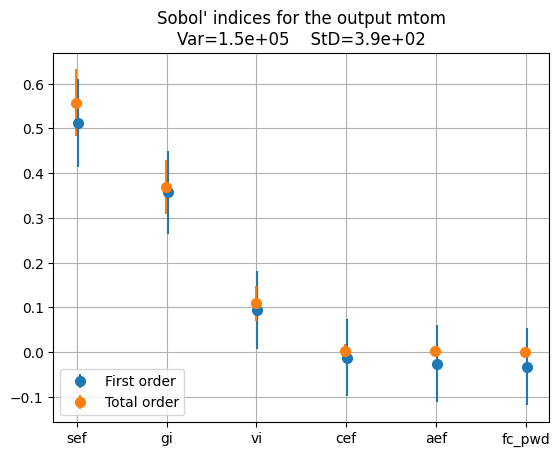
\includegraphics[width=\textwidth]{Images_Ayoub/Problem2/UseCase2/Sobol_Indices/mtom.png}
        \caption{MTOM}
        \label{fig:mtom}
    \end{subfigure}
    \hfill
    \begin{subfigure}[b]{0.45\textwidth}
        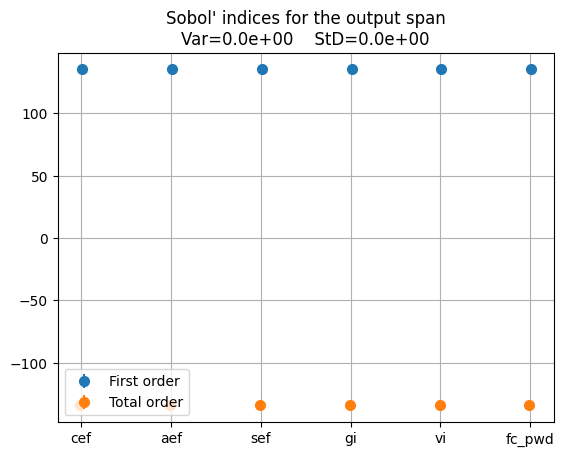
\includegraphics[width=\textwidth]{Images_Ayoub/Problem2/UseCase2/Sobol_Indices/span.png}
        \caption{Span}
        \label{fig:span}
    \end{subfigure}

    \vspace{10pt} % Espacement vertical entre les lignes

    \begin{subfigure}[b]{0.45\textwidth}
        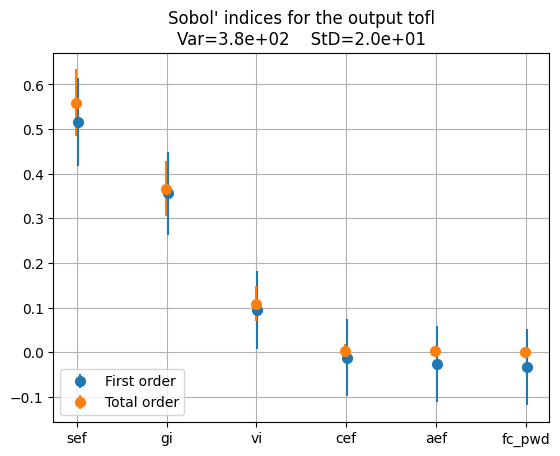
\includegraphics[width=\textwidth]{Images_Ayoub/Problem2/UseCase2/Sobol_Indices/tofl.png}
        \caption{TOFL}
        \label{fig:tofl}
    \end{subfigure}
    \hfill
    \begin{subfigure}[b]{0.45\textwidth}
        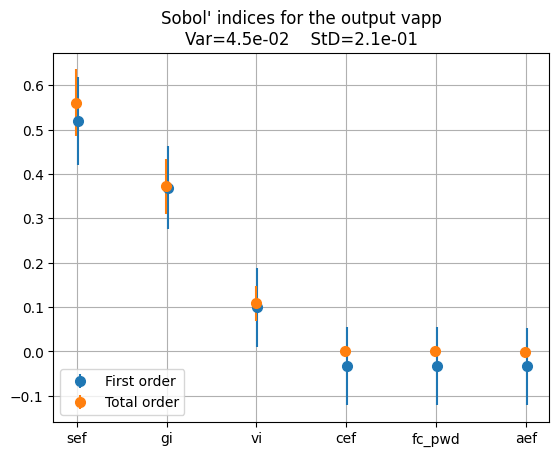
\includegraphics[width=\textwidth]{Images_Ayoub/Problem2/UseCase2/Sobol_Indices/vapp.png}
        \caption{Vapp}
        \label{fig:vapp}
    \end{subfigure}

    \vspace{10pt} % Espacement vertical entre les lignes

    \begin{subfigure}[b]{0.45\textwidth}
        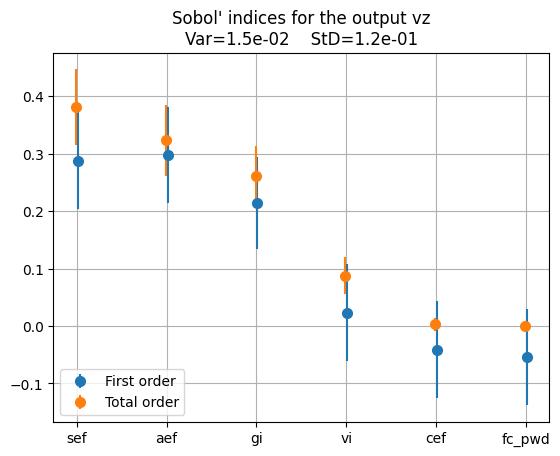
\includegraphics[width=\textwidth]{Images_Ayoub/Problem2/UseCase2/Sobol_Indices/vz.png}
        \caption{Vz}
        \label{fig:vz}
    \end{subfigure}
    \hfill
    \begin{subfigure}[b]{0.45\textwidth}
        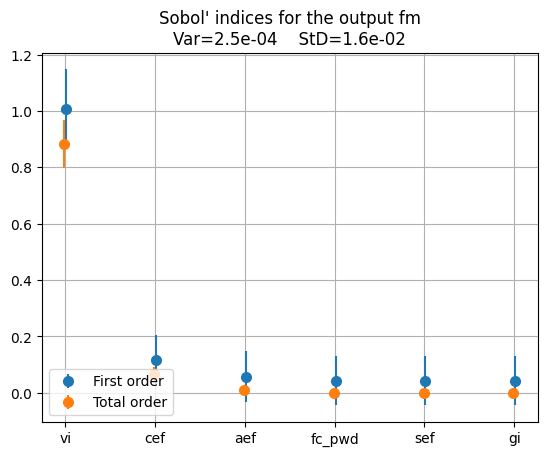
\includegraphics[width=\textwidth]{Images_Ayoub/Problem2/UseCase2/Sobol_Indices/fm.png}
        \caption{FM}
        \label{fig:fm}
    \end{subfigure}

    \caption{Indices de Sobol pour différentes sorties du modèle de substitut.}
    \label{fig:sobol_indices}
\end{figure}


\begin{itemize}
    \item Les sorties (\texttt{MTOM}, \texttt{Span}, \texttt{TOFL}, \texttt{Vapp}, \texttt{Vz}, \texttt{FM}) présentent des sensibilités variées vis-à-vis des paramètres \texttt{sef}, \texttt{gi}, \texttt{vi}, \texttt{cef}, \texttt{aef} et \texttt{fc\_pwd}.
    \item Pour \texttt{MTOM}, le paramètre \texttt{sef} domine clairement la contribution à la variance, suivi par \texttt{gi}, tandis que les autres paramètres ont un impact négligeable.
    \item Pour \texttt{Span}, les indices de Sobol sont incohérents (valeurs extrêmes positives et négatives), ce qui suggère une sortie constante ou une absence de sensibilité significative.
    \item \texttt{TOFL} et \texttt{Vapp} présentent une forte dépendance aux paramètres \texttt{sef} et \texttt{gi}, avec des indices totaux systématiquement supérieurs aux indices de premier ordre, indiquant l'existence d'interactions notables entre ces paramètres.
    \item Pour \texttt{Vz}, l’influence est plus répartie : \texttt{sef} et \texttt{aef} contribuent de manière comparable, suivis par \texttt{gi} et \texttt{vi}.
    \item Enfin, la sortie \texttt{FM} est presque entièrement déterminée par le paramètre \texttt{vi}, qui présente un indice total très élevé, traduisant une dépendance quasi exclusive sans contribution notable des autres paramètres.
    \item Dans l’ensemble, la majorité des sorties sont fortement influencées par un petit nombre de paramètres dominants (\texttt{sef}, \texttt{gi}, \texttt{vi}), et les différences entre indices totaux et de premier ordre révèlent l’importance des effets d’interaction pour certaines sorties.
\end{itemize}

\subsection{Case with $x_{\text{opt}}$}

% Introducing the analysis with fixed x_opt
Ici, nous cherchons à effectuer les mêmes étapes que précédemment, mais en fixant \( \mathbf{x} \) à \( \mathbf{x}_{\text{opt}} \) obtenu dans le Problème 1 à l'aide d'un modèle de substitut. Par souci de concision, nous présentons uniquement le Use Case 1. Un nouveau modèle de substitut a été entraîné, et un espace d'incertitude a été généré pour estimer des quantités telles que les moyennes, les variances, les coefficients de variation, et autres métriques pertinentes.

% Defining the subsection for uncertainty space
\subsubsection{Surrogate Model pour le Use Case 1 avec \( \mathbf{x}_{\text{opt}} \)}

% Describing the uncertainty space analysis
Pour évaluer l'impact des incertitudes sur les sorties du modèle lorsque \( \mathbf{x} \) est fixé à \( \mathbf{x}_{\text{opt}} \), nous avons entraîné un nouveau modèle de substitut pour le Use Case 1 en suivant la même méthodologie que précédemment, en utilisant la classe \texttt{SurrogateDiscipline} avec la méthode \texttt{RBFRegressor}. Le modèle de substitut approxime la fonction \( \mathbf{u} \mapsto f(\mathbf{x}_{\text{opt}}, \mathbf{u}) \), où \( \mathbf{u} \) représente les paramètres incertains (\texttt{cef}, \texttt{sef}, \texttt{aef}, etc.) définis par leurs distributions de probabilité respectives (par exemple, distributions triangulaires \( T(0.99, 1.1, 1.03) \)).


\subsubsection{Estimatiion des quantités d'intérêt}

\subsubsubsection{Distrubtion}
\begin{figure}[H]
    \centering
    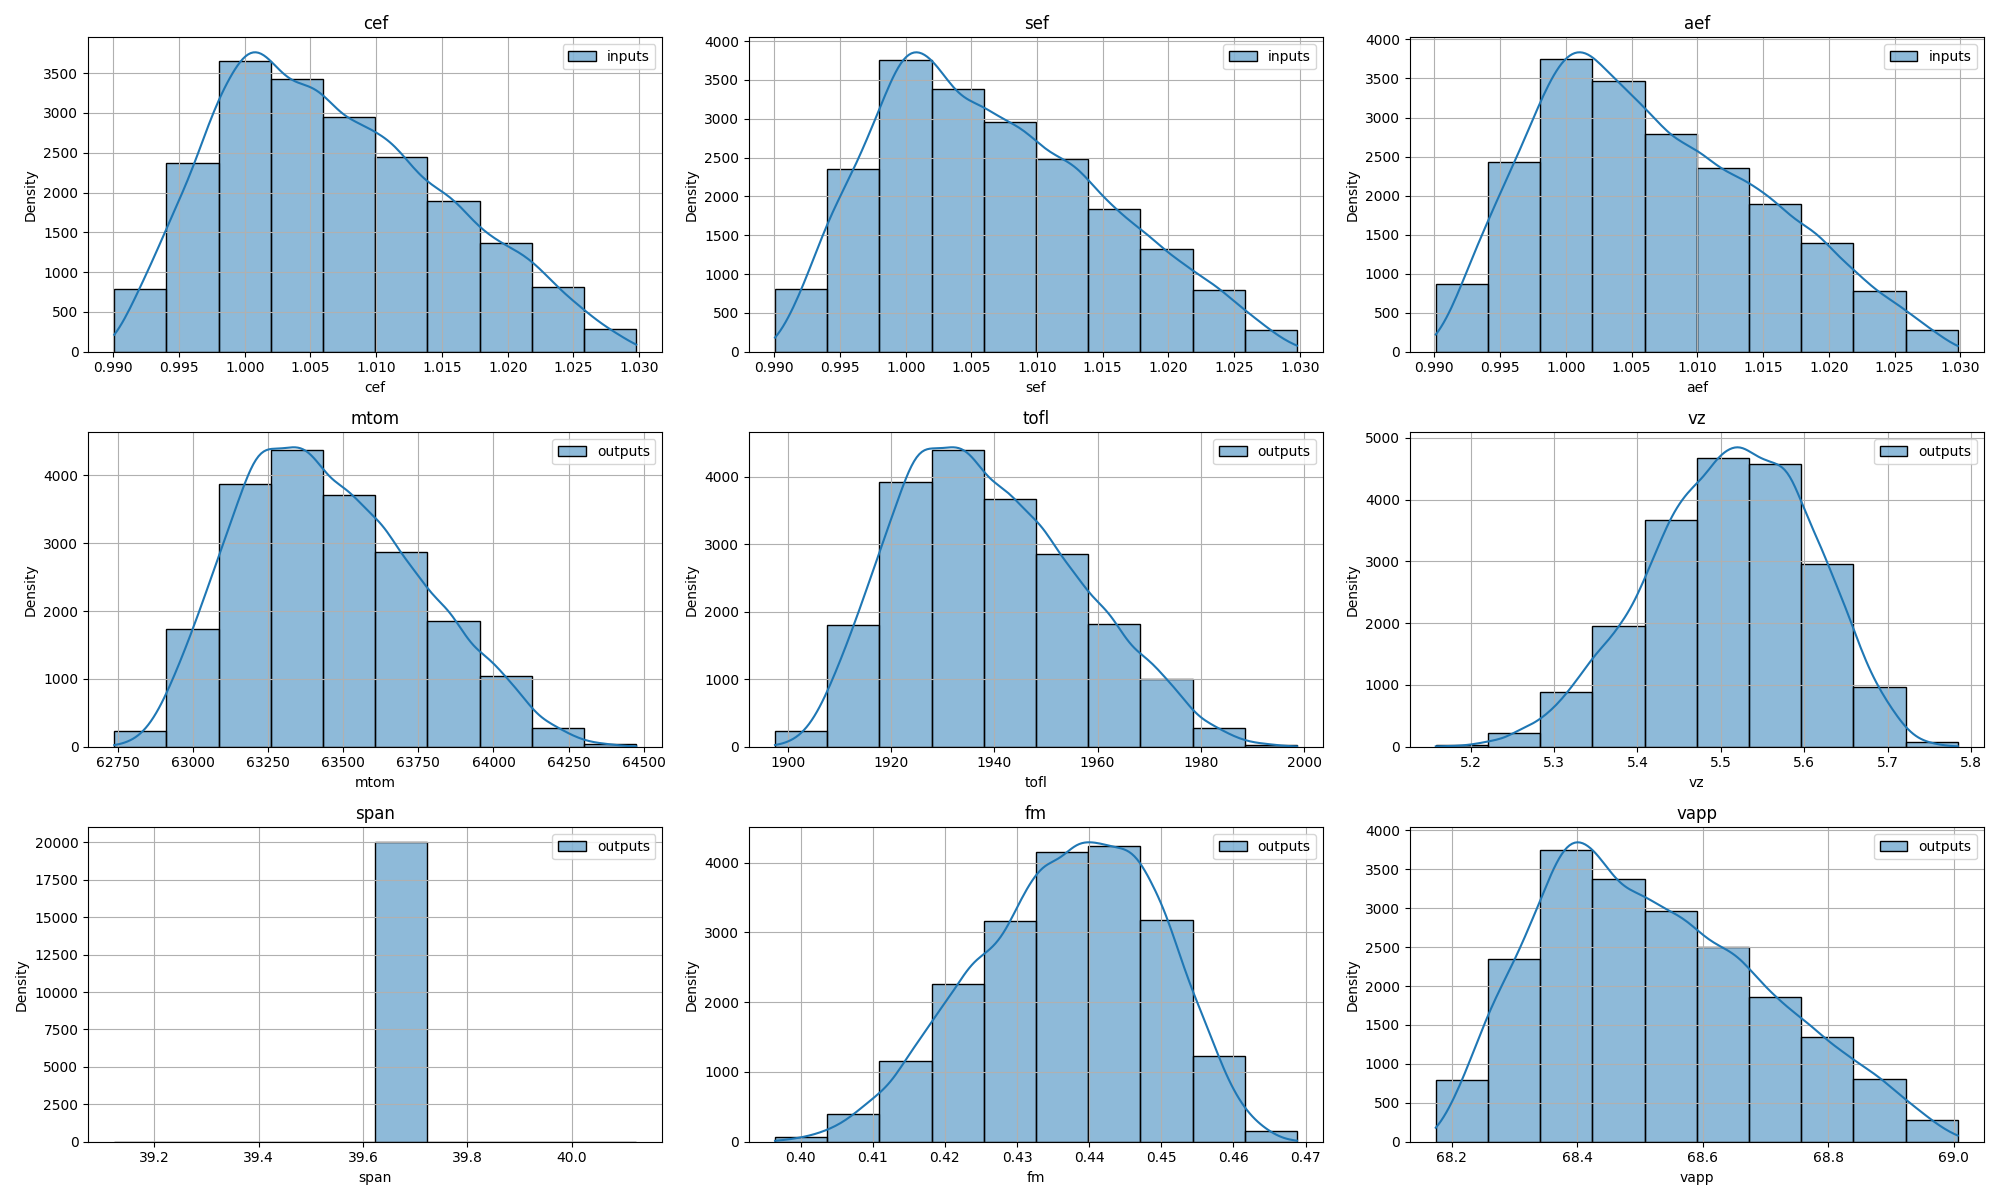
\includegraphics[width=0.9\linewidth]{Images_Ayoub/Problem2/X_opt/Estimating_Quantities/Input_Output_Distributions/image.png}
    \caption{Distribution des échantillons générés pour chaque paramètre incertain (en haut) et distribution des sorties du modèle de substitut (en bas) pour les 20000 échantillons.}
    \label{fig:enter-label}
\end{figure}
%% Partie Ayoub Fin 


\subsubsubsection{Estimation des moyennes et variations et Coefficients de variation}
\begin{table}[h]
\centering
\caption{Paramètres de l'aéronef : moyennes, variances, coefficients de variation et intervalles interquartiles corrigés}
\begin{tabular}{l S[table-format=5.5e1] S[table-format=3.5e1] S[table-format=1.3] S[table-format=1.4]}
\toprule
\textbf{Paramètre} & \textbf{Moyenne} & \textbf{Variance} & \textbf{CV (\%)} & \textbf{IQ} \\
\midrule
MTOM (\si{\kilo\gram}) & 6.3457e4 & 8.9973e4 & 0.473 & 0.0034 \\
TOFL (\si{\meter}) & 1.9391e3 & 3.0361e2 & 0.899 & 0.0065 \\
Vz (\si{\meter\per\second}) & 5.5103e0 & 9.4520e-3 & 1.764 & 0.0124 \\
Span (\si{\meter}) & 3.9623e1 & 0.0000e0 & 0.000 & 0.0000 \\
Length (\si{\meter}) & 3.2000e1 & 5.0487e-29 & 0.000 & 0.0000 \\
FM & 4.3691e-1 & 1.5517e-4 & 2.851 & 0.0206 \\
Vapp (\si{\knot}) & 6.8523e1 & 3.1324e-2 & 0.258 & 0.0019 \\
CEF & 1.0067e0 & 7.1781e-5 & 0.842 & 0.0063 \\
AEF & 1.0066e0 & 7.2384e-5 & 0.845 & 0.0064 \\
SEF & 1.0067e0 & 7.1464e-5 & 0.839 & 0.0063 \\
\bottomrule
\end{tabular}
\end{table}

\begin{figure}[H]
    \centering
    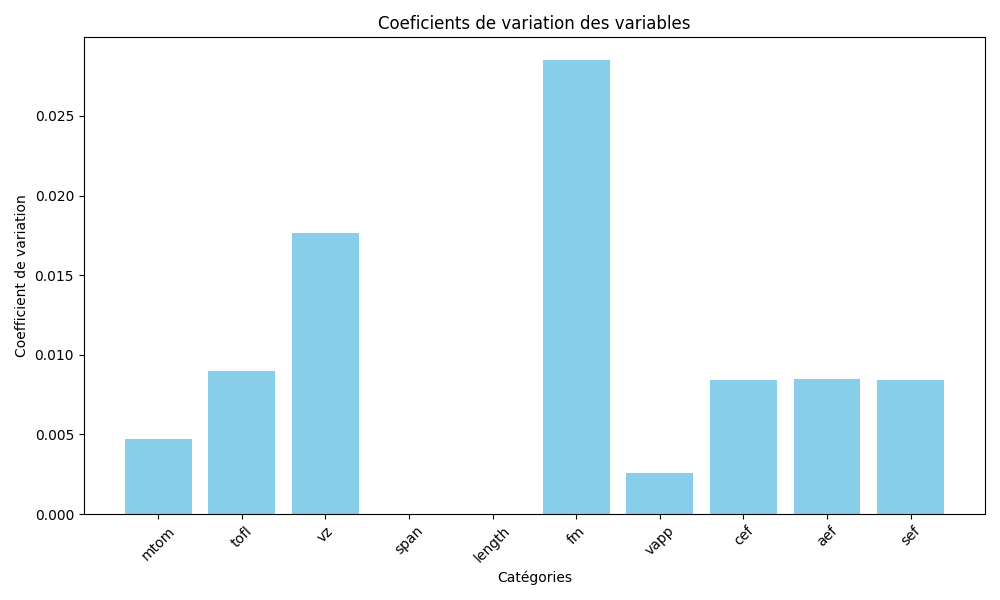
\includegraphics[width=0.9\linewidth]{Images_Ayoub/Problem2/X_opt/Estimating_Quantities/Coefficient_De_Variation/Coefficient_Var.png}
\caption{Coefficients de variation des différentes variables}
    \label{fig:enter-label}
\end{figure}

\subsubsubsection{Indices de Sobol pour le cas $x_{\text{opt}}$}

\begin{figure}[H]
    \centering
    \begin{subfigure}[b]{0.45\textwidth}
        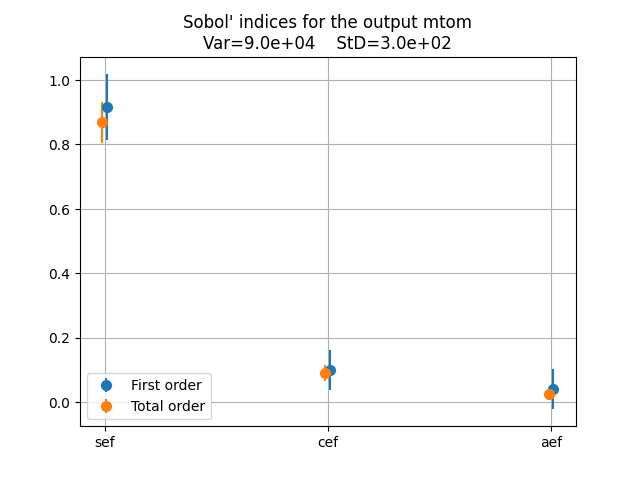
\includegraphics[width=\textwidth]{Images_Ayoub/Problem2/X_opt/Sobol_Indices/mtom.png}
        \caption{MTOM}
        \label{fig:mtom}
    \end{subfigure}
    \hfill
    \begin{subfigure}[b]{0.45\textwidth}
        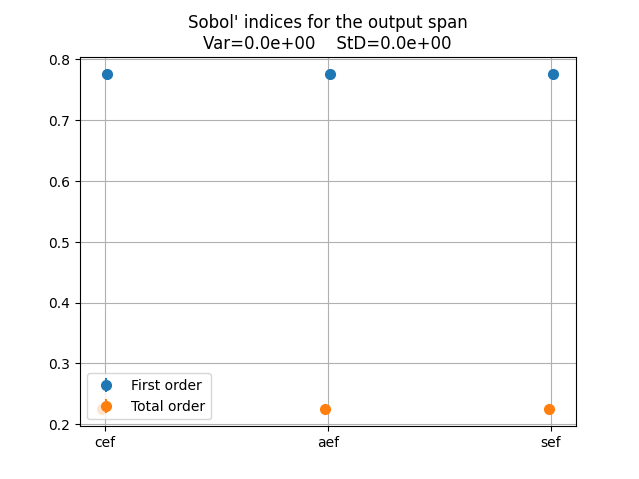
\includegraphics[width=\textwidth]{Images_Ayoub/Problem2/X_opt/Sobol_Indices/span.png}
        \caption{Span}
        \label{fig:span}
    \end{subfigure}

    \vspace{10pt} % Espacement vertical entre les lignes

    \begin{subfigure}[b]{0.45\textwidth}
        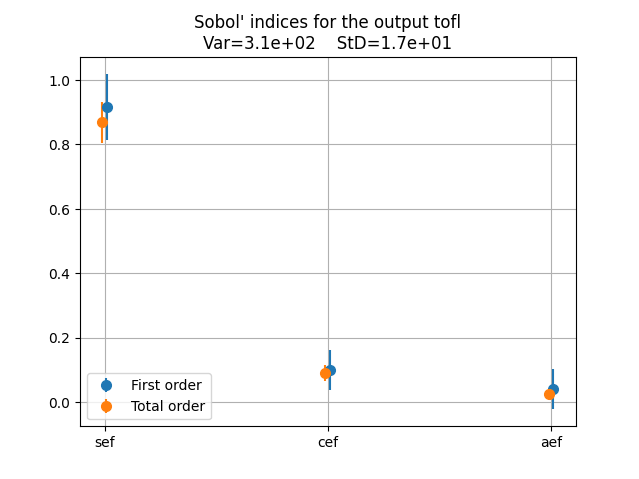
\includegraphics[width=\textwidth]{Images_Ayoub/Problem2/X_opt/Sobol_Indices/tofl.png}
        \caption{TOFL}
        \label{fig:tofl}
    \end{subfigure}
    \hfill
    \begin{subfigure}[b]{0.45\textwidth}
        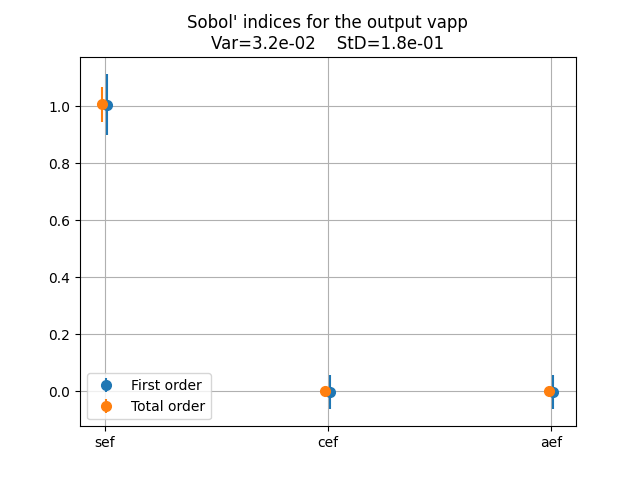
\includegraphics[width=\textwidth]{Images_Ayoub/Problem2/X_opt/Sobol_Indices/vapp.png}
        \caption{Vapp}
        \label{fig:vapp}
    \end{subfigure}

    \vspace{10pt} % Espacement vertical entre les lignes

    \begin{subfigure}[b]{0.45\textwidth}
        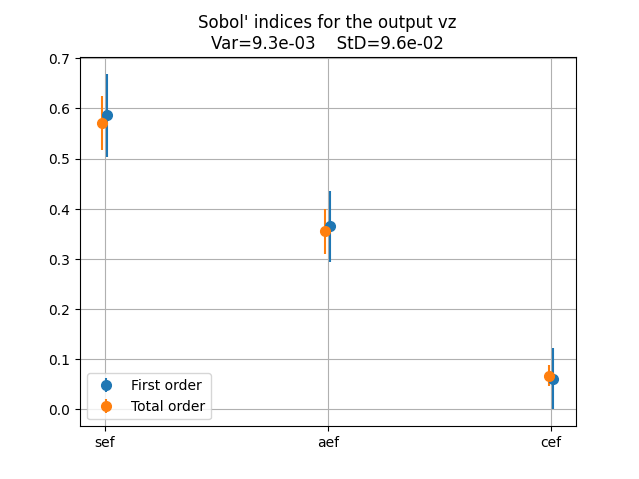
\includegraphics[width=\textwidth]{Images_Ayoub/Problem2/X_opt/Sobol_Indices/vz.png}
        \caption{Vz}
        \label{fig:vz}
    \end{subfigure}
    \hfill
    \begin{subfigure}[b]{0.45\textwidth}
        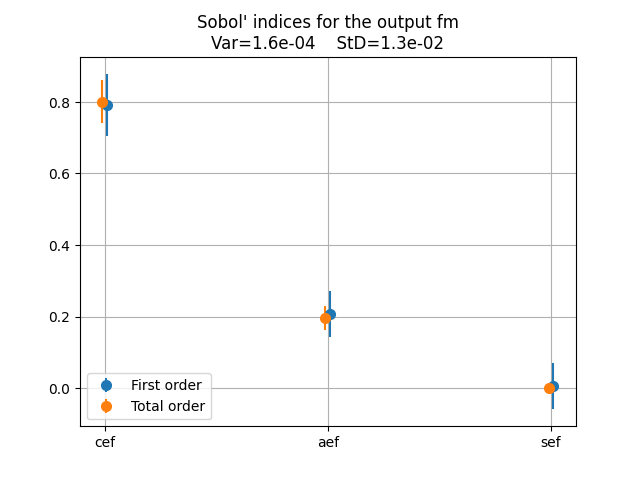
\includegraphics[width=\textwidth]{Images_Ayoub/Problem2/X_opt/Sobol_Indices/fm.png}
        \caption{FM}
        \label{fig:fm}
    \end{subfigure}

    \caption{Indices de Sobol pour différentes sorties du modèle de substitut.}
    \label{fig:sobol_indices}
\end{figure}


\section{Problème 3}
% Rapport à rendre le 22 (au plus tard)
Dans cette troisième partie, comme dans la réalité, nous souhaitons intégrer les incertitudes dans notre problème d’optimisation. Nous choisissons un critère où l'objectif est de minimiser l’espérance de la masse, en considérant que toutes les paramettres (u) et variables de sortie deviennent aléatoires.

Afin de mieux respecter les contraintes malgré la présence d’incertitudes, nous ajoutons également un terme correspondant à deux fois l’écart-type, appliqué sur l’espérance des contraintes. Cela signifie que si les variables des contraintes suivent une loi normale, alors ces contraintes seront satisfaites avec une probabilité de 95\%.

Le problème initial devient donc le suivant :


\begin{align}
    \begin{cases}
        \min_{x} \ \mathbb{E}[f(x,U)] \\
        \text{s.c. } \ \mathbb{E}[g(x,U)] + 2S[g(x,U)] \leq 0
    \end{cases}
\end{align}

Nous allons ainsi proposer trois méthodes, impliquant des charges de calcul différentes, pour résoudre ce problème de manière numérique.


\subsection{Méthode de dévéloppement de Taylor}
Par le dévéloppement de Taylor:
\begin{equation}
    f(x,U) \approx f(x,\mathbb{E}[U]) + \frac{\partial f(x,\mathbb{E}[U])}{\partial U}(U - \mathbb{E}[U])
\end{equation}
On prend l'espérance, en rendant compte que $\mathbb{E}[U - \mathbb{E}[U]] = 0$ donc $\mathbb{E}[f(x,U)]\approx f(x,\mathbb{E}[U])$ et $\mathbb{E}[g(x,U)]\approx g(x,\mathbb{E}[U])$. On a donc 
\begin{align*}
    S[g(x,U)] &= \mathbb{E}[g(x,U) - \mathbb{E}[g(x,U)]]^2 \\ &\approx \mathbb{E}[g(x,U) - g(x,\mathbb{E}[U])]^2 \\
    &= \mathbb{E}\left[\frac{\partial g(x,\mathbb{E}[U])}{\partial U}(U - \mathbb{E}[U])\right]^2 \\
    &= \left( \frac{\partial g(x,\mathbb{E}[U])}{\partial U} \right)^2\mathbb{E}\left[U - \mathbb{E}[U]\right]^2 \\
    &= \left( \frac{\partial g(x,\mathbb{E}[U])}{\partial U} \right)^2 \text{Var}(U)
\end{align*}
Le problème d'optimimisation se ramène à la version linéarisée: 
\begin{align*}
    \begin{cases}
        \min_{x} f(x,\mathbb{E}[U]) \\
        \text{ s.c.    }  g(x,\mathbb{E}[U]) + 2\frac{\partial g(x,\mathbb{E}[U])}{\partial U}\sqrt{\text{Var}(U)} \leq 0
    \end{cases}
\end{align*}

Nous obtenons donc le résultat suivant.

- Cas d'usage 1:  
\begin{figure}[H]
    \centering
    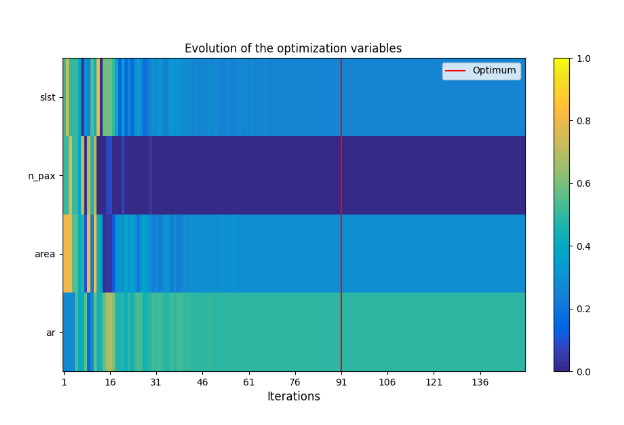
\includegraphics[width=0.45\linewidth]{Images_case_1/p3u1_taylor1.png}
    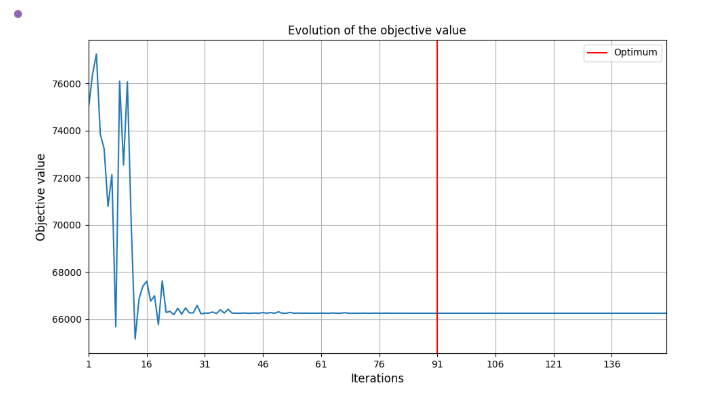
\includegraphics[width=0.45\linewidth]{Images_case_1/p3u1_taylor3.png}
    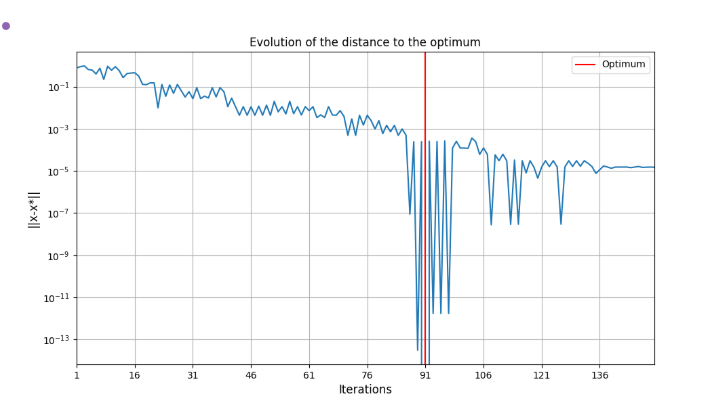
\includegraphics[width=0.45\linewidth]{Images_case_1/p3u1_taylor4.png}
    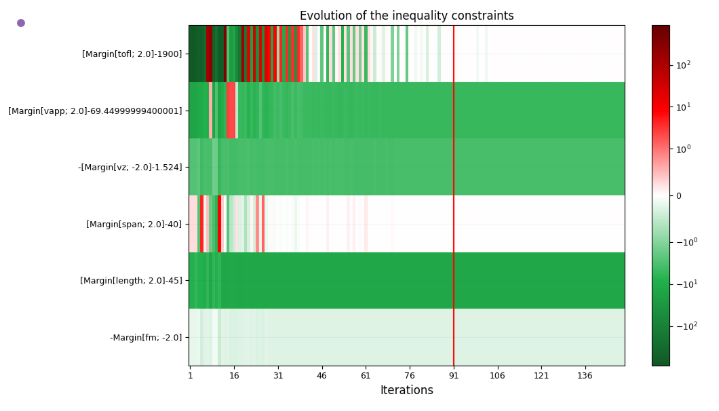
\includegraphics[width=0.45\linewidth]{Images_case_1/p3u1_taylor2.png}
    \caption{Evolution d'optimisation du cas 1 par la méthode de dévéloppement de Taylor}
    \label{fig:p3u2_taylor}
\end{figure}

- Cas d'usage 2:  
\begin{figure}[H]
    \centering
    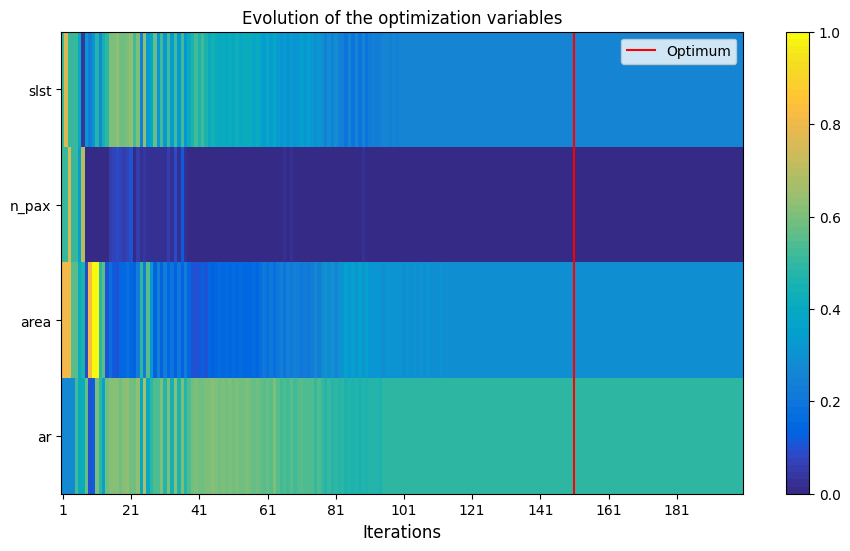
\includegraphics[width=0.45\linewidth]{Images_case_2/p3u2_taylor.png}
    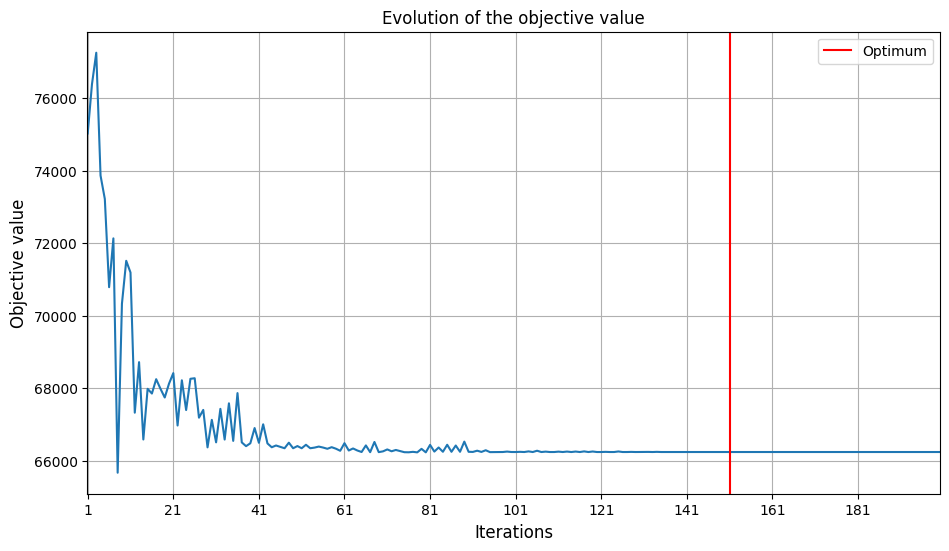
\includegraphics[width=0.45\linewidth]{Images_case_2/p3u2_taylor_evol_obj.png}
    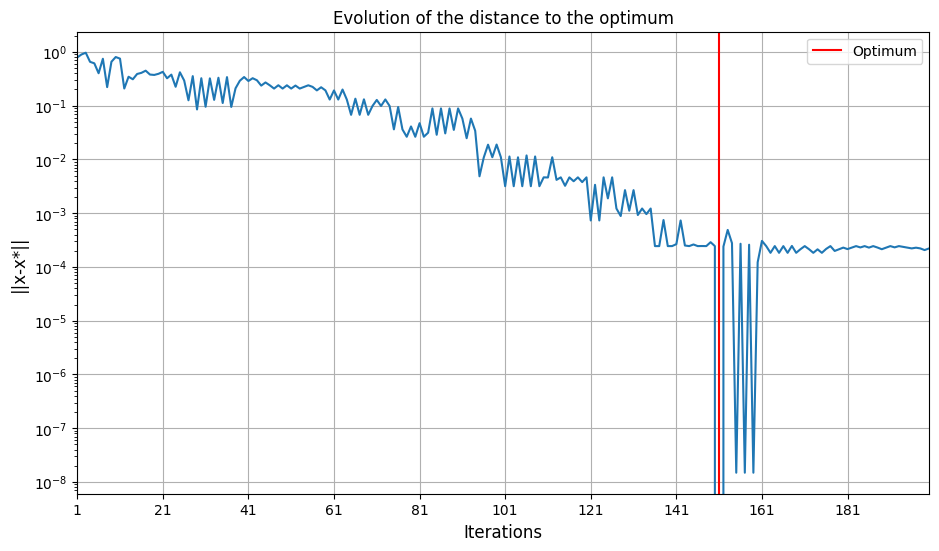
\includegraphics[width=0.45\linewidth]{Images_case_2/p3u2_taylor_evol_dist.png}
    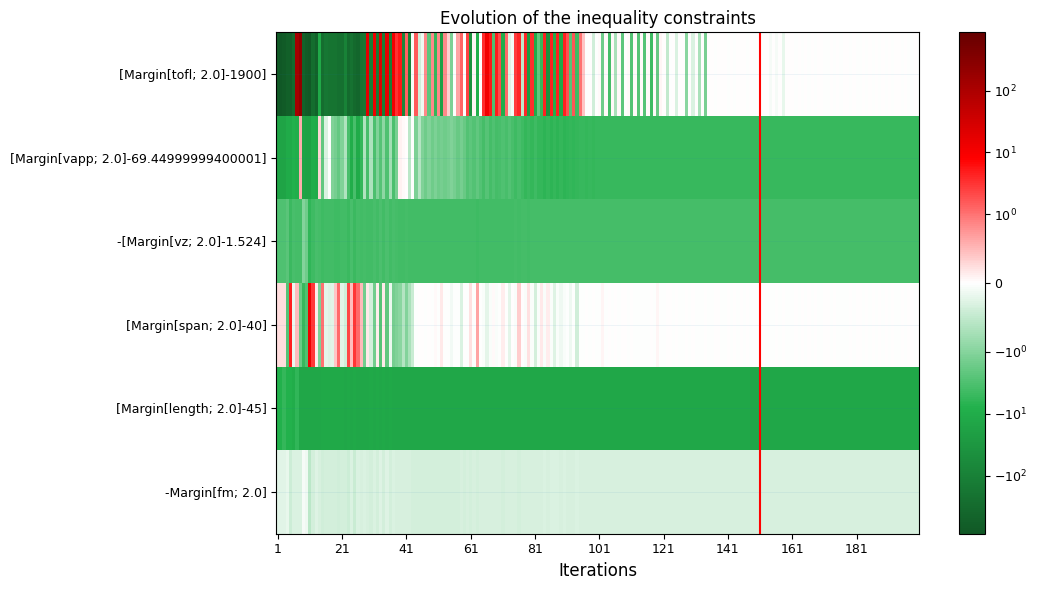
\includegraphics[width=0.45\linewidth]{Images_case_2/p3u2_taylor_evol_constraint.png}
    \caption{Evolution d'optimisation du cas 2 par la méthode de dévéloppement de Taylor}
    \label{fig:p3u2_taylor}
\end{figure}

L’optimisation a été correctement réalisée et la solution a bien convergé. Nous avons vérifié cela dans le scénario réel de la discipline concernée, et toutes les contraintes sont respectées.

% f(g(x,u)) \approx g(x,\mathbb{E}(U)) + \frac{\partial g}{\partial u}(x, \mathbb{E}(U))(\mathbb{E}(U)-u) + \frac{1}{2} \frac{\partial^2 g}{\partial u^2}(x, \mathbb{E}(U))(\mathbb{E}(U)-u)^2



% Petits schémas :
% \text{Courbe de Gauss (ou densité normale) avec abscisse à 95\% et 1900}

\subsection{Méthode par surrogate direct}

De manière similaire au problème 1, notre première idée consiste à construire un modèle surrogate direct $\hat{f}$ prenant à la fois $x$ et $u$ comme variables d’entrée, et renvoyant l’objectif et les contraintes. Une fois ce modèle surrogate validé, l’optimisation peut être réalisée sur $x$ en utilisant une approche de Monte Carlo sur $u$.

On peut alors reformuler le problème sous la forme suivante :

\begin{align*}
    \begin{cases}
        \displaystyle \min_{x} \ \frac{1}{N} \sum_{i=1}^{N} \hat{f}(x, u_i) \\
        \text{s.c.} \ \displaystyle \frac{1}{N} \sum_{i=1}^{N} \hat{g}(x, u_i) + 2 S[\hat{g}(x, u_{1:N})] \leq 0 \\
        \left\| (f, g) - (\hat{f}, \hat{g}) \right\| < \epsilon
    \end{cases}
\end{align*}

où l’écart-type est défini par :

\begin{align*}
    S[\hat{g}(x, u_{1:N})] = \sqrt{ \frac{1}{N-1} \sum_{i=1}^{N} \left( \hat{g}(x, u_i) - \frac{1}{N} \sum_{j=1}^{N} \hat{g}(x, u_j) \right)^2 }
\end{align*}

Cette approche permet ainsi de prendre en compte la variabilité induite par $u$ dans l’évaluation des contraintes, via la moyenne et l’écart-type estimés à partir d’un échantillonnage Monte Carlo.

Comme $\hat{f}$ est un modèle substitut surrogate, l’évaluation sur ce modèle est relativement peu coûteuse. Il est donc possible de choisir une taille d’échantillon N suffisamment grande, ce qui permet à la moyenne empirique de bien approcher l’espérance théorique.

Cependant, une difficulté subsiste dans des situations réalistes où la dimension de la variable d’entrée x est souvent élevée. De plus, la construction d’un modèle substitut nécessite généralement l’ajout de variables supplémentaires, telles que u, ce qui augmente encore la dimension du problème. Étant donné que l’évaluation du modèle direct est particulièrement coûteuse, il n’est généralement pas possible de générer un grand volume de données d’entraînement. Dans ce contexte, il devient difficile pour le modèle substitut de représenter fidèlement le comportement du modèle direct.

- Cas d'usage 2 
\begin{figure}[H]
    \centering
    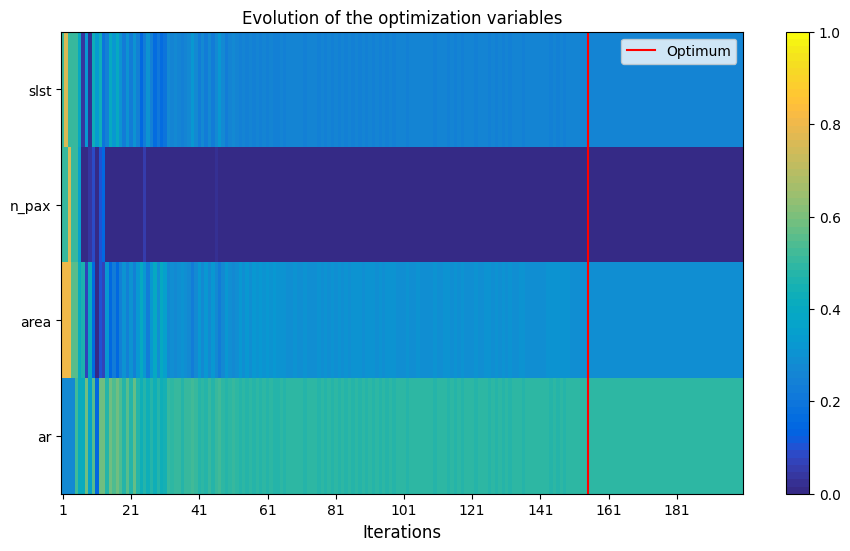
\includegraphics[width=0.45\linewidth]{Images_case_2/p3u2_direct.png}
    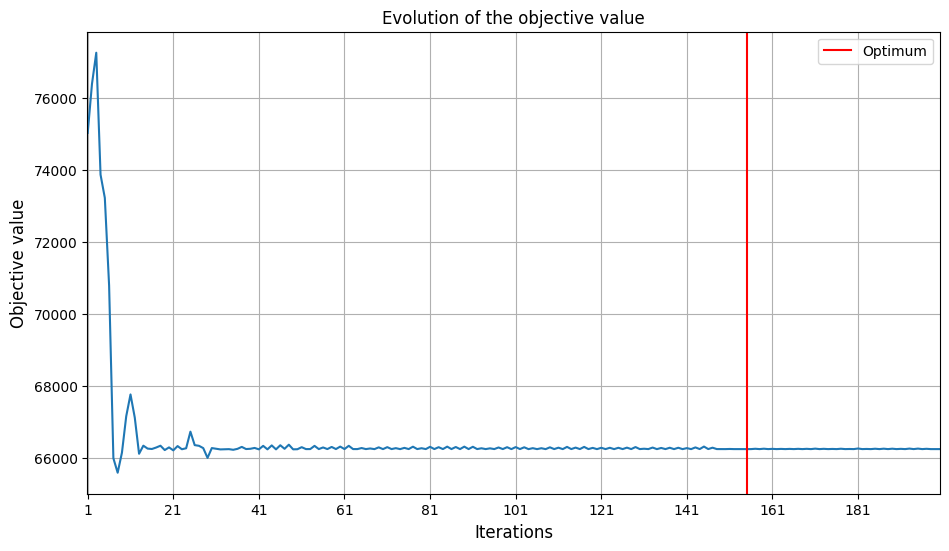
\includegraphics[width=0.45\linewidth]{Images_case_2/p3u2_direct_evol_obj.png}
    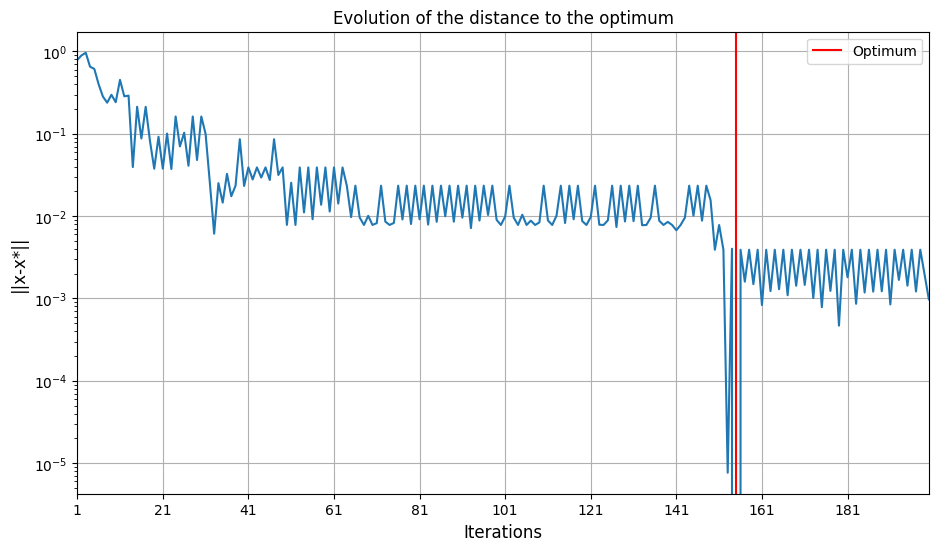
\includegraphics[width=0.45\linewidth]{Images_case_2/p3u2_direct_evol_dist.png}
    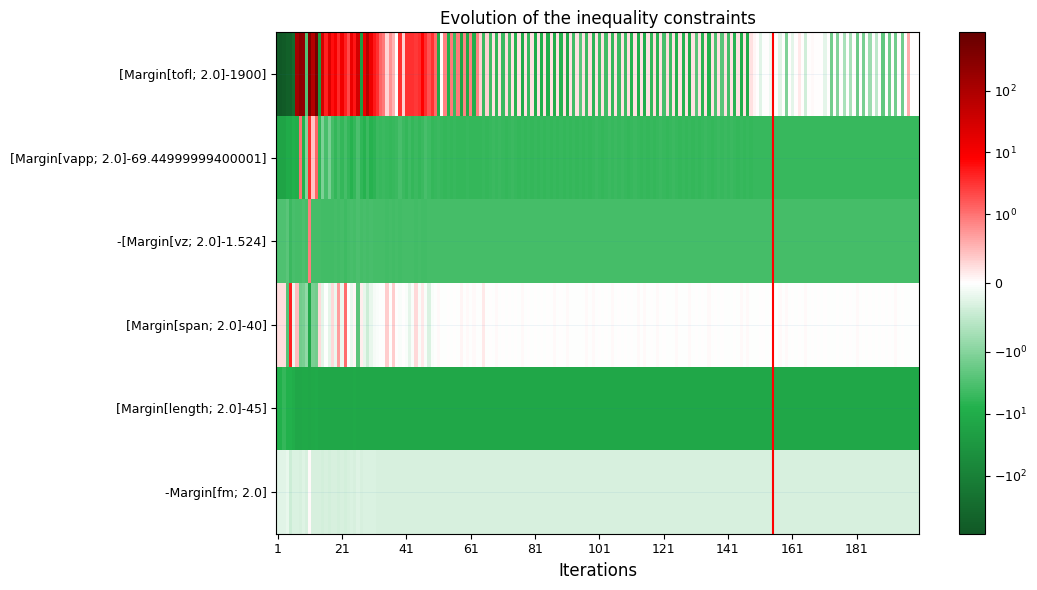
\includegraphics[width=0.45\linewidth]{Images_case_2/p3u2_direct_evol_constraint.png}
    \caption{Evolution d'optimisation du cas d'usage 2 par la méthode de surrogate direct}
    \label{fig:p3u2_direct}
\end{figure}

Malheureusement, malgré le changement des différentes méthodes de régression, lorsque nous testons les résultats de ces méthodes sur le modèle réel, la contrainte TOFL n’est toujours pas respectée.

\begin{figure}[H]
    \centering
    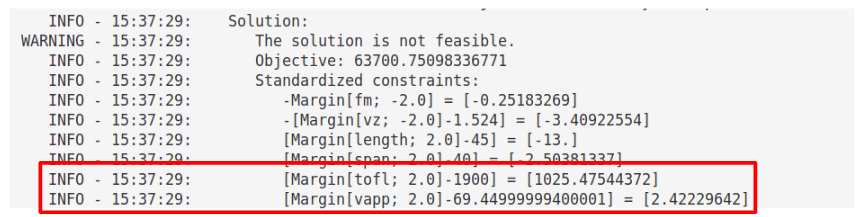
\includegraphics[width=0.85\linewidth]{Images_case_2/contraint_non_verif.png}
    \caption{Contraint tolf n'est pas vérifié}
    \label{fig:enter-label}
\end{figure}

La raison pourrait être que le $R^{2}$ du modèle surrogate n’est pas parfait (0,93), et que la solution tombe dans une zone de mauvaise prédiction. Cela reste à vérifier.




\subsection{Méthode par surrogate local itératif}
Dans la continuité des approches précédentes, nous proposons une méthode par surrogate local itératif visant à surmonter certaines limitations des méthodes antérieures. Contrairement à l’approximation linéaire de la méthode de Taylor, qui peut être trop simplificatrice, et à la méthode par surrogate direct, qui pâtit de la complexité liée à la forte dimensionnalité de $x$ et $U$, cette approche itérative reconstruit un modèle surrogate à chaque itération. Cela permet d’affiner progressivement la représentation du modèle en se focalisant sur les régions pertinentes de l’espace des paramètres. L’algorithme de cette méthode est détaillé dans le tableau 1.

Plutôt que de construire un modèle surrogate global intégrant simultanément $x$ et $u$ comme variables d’entrée, cette méthode adopte une stratégie séquentielle. À chaque itération $k$, un modèle surrogate local $\hat{f}_{x_k}(u)$ est construit en fixant la variable $x$ à $x_k$. Ce modèle approxime localement la fonction objectif $f$ en fonction de la variable aléatoire $u$.

La valeur de $f$ pour $x_k$ est ensuite estimée par échantillonnage Monte Carlo de $u$ à l’aide du surrogate. La valeur suivante, $x_{k+1}$, est déterminée en minimisant cette approximation locale. Ce processus itératif se poursuit jusqu’à satisfaire un critère de convergence ou atteindre un nombre maximal d’itérations.

Cette approche réduit la quantité de données nécessaires à chaque itération et permet de mieux maîtriser le coût computationnel, notamment pour les problèmes de haute dimension.
\vspace{0.5em}
\subsubsection{Algorithme.}
Voici le pseudo-code de cette approche séquentielle :

\begin{algorithm}[H]
\caption{Optimisation séquentielle avec surrogate local}
\begin{algorithmic}[1]
    \State Initialiser $x_0 = x_{\text{défaut}}$
    \While{$k < \textit{MaxIter}$ \&\& critère de convergence ne atteint pas}
        \State Échantillonner $u_1, \dots, u_N \sim P(u)$
        \State Construire un modèle surrogate $\hat{f}_{x_k}(u)$ en fixant $x = x_k$
        \State Calculer $x_{k+1} = \arg\min_x \; \mathbb{E}_{u} \left[ \hat{f}_x(u) \right]$ par moyenne Monte Carlo
    \EndWhile
    \State \Return $x_{k+1}$
\end{algorithmic}
\end{algorithm}

\vspace{0.5em}

Cette méthode présente plusieurs avantages. Elle nécessite moins de données d’apprentissage à chaque itération, car le modèle substitut est construit localement pour une valeur donnée de $x$. Elle est ainsi moins sensible à la dimension de la variable d’entrée $x$, ce qui la rend bien adaptée aux problèmes de forte dimension où l’évaluation du modèle direct est coûteuse. De plus, le coût d’apprentissage et d’optimisation reste réduit à chaque itération. Cette approche séquentielle permet également d’ajuster dynamiquement le surrogate en fonction de l’avancement de l’optimisation, ce qui peut améliorer la stabilité du processus et la qualité des solutions obtenues, notamment lorsque les ressources de calcul sont limitées.

\vspace{0.5em}

En revanche, cette méthode présente certaines limitations. Elle peut nécessiter un nombre important d’itérations pour converger, en particulier si la fonction objective est fortement non linéaire ou si elle comporte plusieurs minima locaux. Par ailleurs, les interactions entre $x$ et $u$ sont prises en compte de manière plus approximative, puisque le surrogate est localisé autour de $x_k$ et ne modélise pas globalement la dépendance de $f$ à $x$. La qualité de la solution obtenue dépend donc directement de la précision locale des surrogates successifs. 

Nous obtenons donc le résultat suivant.


- Cas d'uasge 1: 
\begin{figure}[H]
    \centering
    \includegraphics[width=0.45\linewidth]{Images_case_1/p3u1_surrogate.png}
    \includegraphics[width=0.45\linewidth]{Images_case_1/p3u1_surrogate1.png}
    \includegraphics[width=0.45\linewidth]{Images_case_1/p3u1_surrogate2.png}
    \includegraphics[width=0.45\linewidth]{Images_case_1/p3u1_surrogate3.png}
    \caption{Evolution d'optimisation du cas d'usage 1 par la méthode de surrogate modèle iteratif}
    \label{fig:p3u2_iter_c1}
\end{figure}

- Cas d'uasge 2: 
\begin{figure}[H]
    \centering
    \includegraphics[width=0.45\linewidth]{Images_case_2/p3u2_iter.png}
    \includegraphics[width=0.45\linewidth]{Images_case_2/p3u2_iter_evol_obj.png}
    \includegraphics[width=0.45\linewidth]{Images_case_2/p3u2_iter_evol_dist.png}
    \includegraphics[width=0.45\linewidth]{Images_case_2/p3u2_iter_evol_constraint.png}
    \caption{Evolution d'optimisation du cas d'usage 2 par la méthode de surrogate modèle iteratif}
    \label{fig:p3u2_iter_c2}
\end{figure}

L’optimisation a été correctement réalisée et la solution obtenue est très proche de celle de la première méthode. Nous avons vérifié ce résultat dans un scénario réel propre à la discipline concernée, et toutes les contraintes sont respectées.

\subsection{Visualiation de l'aéronef optimisé par des modèles surrogate}


\begin{figure}[H]
    \centering
    \includegraphics[width=0.45\linewidth]{Images_case_1/aircraft_poly.png}
    \includegraphics[width=0.45\linewidth]{Images_case_1/aircraft_ite.png}
    \includegraphics[width=0.45\linewidth]{Images_case_2/aircraft_poly.png}
    \includegraphics[width=0.45\linewidth]{Images_case_2/aircraft_ite.png}
    \caption{Top: Use case 1. Bottom: Use case 2}
    \label{fig:enter-label}
\end{figure}




\section{Conclusion}
Dans ce rapport, nous avons abordé l'optimisation d'un avion de 150 passagers environ, en considérant différents types de carburant et de moteurs, avec pour objectif principal de minimiser la masse maximale au décollage (\textbf{mtom}) tout en respectant les contraintes opérationnelles. À travers les trois problèmes étudiés, nous avons développé et comparé diverses approches de métamodélisation et d'optimisation, en tenant compte des incertitudes inhérentes à la conception aéronautique.

Dans le \textbf{Problème 1}, nous avons construit des métamodèles basés sur \texttt{RBFRegressor} et \texttt{MOERegressor} à partir d'un échantillonnage limité. Le \textbf{Problème 2} a introduit la prise en compte des incertitudes, modélisées par des distributions de probabilité pour les paramètres incertains. Enfin, dans le \textbf{Problème 3}, nous avons proposé trois méthodes pour intégrer les incertitudes dans l'optimisation : le développement de Taylor, le surrogate direct et le surrogate local itératif.

\end{document}\usepackage{algorithm}
\usepackage{algpseudocode}